% Proof-of-Instant-Settlement — Harpo
% Compila com: pdflatex instant-settlement.tex  (2x para refs)
% Dependencias: pacotes padrao (article, amsmath, amssymb, hyperref, booktabs, xcolor, geometry).
% Nenhuma dependencia exotica — proposital, para reprodutibilidade.
\documentclass[11pt]{article}

\usepackage[utf8]{inputenc}
\usepackage[T1]{fontenc}
\usepackage{lmodern}
\usepackage{amsmath,amssymb,amsthm}
\usepackage{booktabs}
\usepackage{xcolor}
\usepackage[margin=1in]{geometry}
\usepackage{microtype}
\usepackage[colorlinks=true,linkcolor=blue,citecolor=blue,urlcolor=blue,breaklinks=true,
  pdftitle={Proof-of-Instant-Settlement: Cryptographically Binding PSP-Attested Instant Payments to Confidential On-Chain State},
  pdfauthor={Juliano Pereira Sales, Marco Tulio Rocha Nascimento},
  pdfsubject={Zero-knowledge proofs, confidential settlement, instant payments},
  pdfkeywords={Groth16, zk-SNARK, Pix, instant payments, confidential transactions, PSP attestation}
]{hyperref}
\usepackage{tikz}
\usetikzlibrary{arrows.meta,positioning,fit,backgrounds}

\newtheorem{property}{Property}
\newtheorem*{assumption}{Assumption}
\newtheorem{theorem}{Theorem}
\newtheorem{corollary}{Corollary}
\newcommand{\Poseidon}{\ensuremath{\mathsf{Poseidon}}}
\newcommand{\Fp}{\ensuremath{\mathbb{F}_p}}
\newcommand{\eeid}{\ensuremath{\mathsf{e2eId}}}
\newcommand{\code}[1]{\texttt{#1}}

\title{\textbf{Proof-of-Instant-Settlement:}\\
Cryptographically Binding PSP-Attested Instant Payments\\
to Confidential On-Chain State}

\author{%
  \begin{tabular}[t]{c}
  Juliano Pereira Sales \\
  \small Harpo \quad\textbar\quad \texttt{harpo-zk} \\
  \small \href{mailto:tzdesing@gmail.com}{tzdesing@gmail.com}
  \end{tabular}
  \and
  \begin{tabular}[t]{c}
  Marco T\'ulio Rocha Nascimento \\
  \small Harpo \quad\textbar\quad \texttt{harpo-zk} \\
  \small \href{mailto:marcotulio.nascimento@gmail.com}{marcotulio.nascimento@gmail.com}
  \end{tabular}
}

\date{\today}

\begin{document}
\maketitle

\begin{abstract}
We present Proof-of-Instant-Settlement, a construction that binds a specific
real-world instant payment --- attested by the regulated payment service
provider (PSP) that observed it --- to a confidential on-chain commitment, so
that a public-EVM contract can verify \emph{that the fiat money settled, for
this exact operation}, without the amount or the counterparties ever appearing
on-chain. The contribution is the binding itself, not new primitives: on-chain
confidentiality layers (Zeto, Railgun, Rayls/Enygma) prove \emph{confidential
transfers} between on-chain accounts, but, to the best of our knowledge, none
of the public-EVM confidential-transfer systems considered here binds its
private state to a real fiat settlement. Our concrete instantiation targets
Brazil's central-bank instant-payment rail (Pix), whose payments carry a unique
rail-level identifier, the \emph{EndToEndId} (E2EID). The construction pairs a
Groth16 circuit, which proves that a commitment opens to the E2EID and terms of
a specific payment, with an attestation oracle that lets the chain verify ---
through an EIP-712 signature from a registered PSP --- that this E2EID
corresponds to a payment the PSP reports as settled and credited. We are precise about what is proved and by whom: the
construction proves a PSP-attested claim about the rail, not the rail's own
cryptographic truth; \S\ref{sec:security} states this trust boundary as the
central fact about the system, not a footnote. The construction is
\emph{two-phase}: a
commitment $c_0$ to the agreed terms is registered when the charge is created,
before any payment exists, and the settlement commitment $c$ is proven to carry
the same amount and charge identifier --- which gives an asset escrow something
to lock onto: the commitment/escrow primitive a delivery-versus-payment
composition needs, though composing it with the payment leg into a single
atomic transition is not itself demonstrated here (\S\ref{sec:futurework}). The
PSP signs over $c_0$ rather than over the amount, so the protocol verifies
\emph{value consistency without the value ever appearing on-chain}. We give the
circuit ($1{,}251$ R1CS constraints), the on-chain verification cost measured on
a live public testnet, the gas of the complete settlement and attestation calls,
and an explicit, honest threat model. We are deliberate about the residual trust:
the oracle replaces ``trust the submitter'' with ``trust a PSP whose key is
registered, whose attestations expire, and whose every attestation is auditable
on-chain'' --- it does \emph{not} remove trust in the PSP. Removing that last
assumption (via a central-bank attestation, dual attestation over an open-banking
API, or zkTLS over the PSP endpoint) is stated as the core open problem. We
additionally report a well-determinedness constraint analysis of the settlement
circuits, a family of
\emph{confidential compliance predicates} bound to a PSP-attested counterparty
commitment, and a post-quantum audit-disclosure channel (ML-KEM, FIPS-203). This
is a research prototype: validated end-to-end on the XDC Apothem testnet, not yet
run in production, with the reference implementation currently maintained by a
single maintainer.
\end{abstract}

\begin{center}
\fbox{\begin{minipage}{0.92\textwidth}
\small
\textbf{What this construction proves, stated as a boundary.}
\emph{Cryptographically}: the same amount and \code{txid} underlie $c_0$ and
$c$ (Property~\ref{prop:twophase}); the settlement tag is deterministic in
\eeid{} under a registered, immutable domain key and single-use within that
domain (Property~\ref{prop:uniqueness}); the counterparty commitment
consistent with the settlement proof is the one the PSP attested, or the
operation does not close (Properties~\ref{prop:settlementbinding}
and~\ref{prop:auth}).
\emph{Institutionally}: a registered PSP attested that it observed this
payment settle and credit, over this $c_0$ and this counterparty commitment
(Assumption~(I1)). \emph{Not proved}: that the central bank's own
infrastructure settled the payment (\S\ref{sec:security} discusses four
candidate paths, none evaluated here); that the attesting PSP is honest, only
that a registered key signed (Property~\ref{prop:auth}); economic
irreversibility of the settlement (\S\ref{sec:reversal}); unlinkability across
operations (\S\ref{sec:security}, ``confidentiality is not unlinkability'');
or soundness under a production-grade trusted setup (\S\ref{sec:security}
states the reference artifacts' setup as a single-contributor, non-MPC ceremony).
\end{minipage}}
\end{center}

\section{Introduction}

Confidential-transfer systems on EVM chains prove, in zero knowledge, that a
private balance update is well-formed (values conserved, ownership valid, no
double-spend). This is by now a commodity: Zeto, Railgun, and the Brazilian
central-bank-adjacent Rayls/Enygma all rely on the same primitive family
(Groth16 or PLONK over BN254/BLS12-381, Pedersen/Poseidon commitments, UTXO or
account models with nullifiers)~\cite{rayls,zeto}. What none of them addresses is
the \emph{link to a real payment rail}: the on-chain proof says nothing about
whether fiat currency actually moved.

\paragraph{Terminology for readers outside Brazil.}
The concrete rail throughout this paper is \emph{Pix}, the instant-payment
system operated by the Central Bank of Brazil (Banco Central do Brasil, Bacen)
since 2020, which settles transfers between accounts at different institutions
in seconds, around the clock, over a central infrastructure called the SPI.
Participants connect to it through regulated \emph{payment service providers}
(PSPs): banks and licensed payment institutions that hold the end-user
accounts. A Pix payment is identified by two strings that this paper relies
on. The \emph{EndToEndId} (E2EID) is a unique identifier assigned when the
payment is initiated and carried end-to-end through the rail; the receiving
PSP learns it when the funds are credited, and the SPI enforces its
uniqueness. The \emph{txid} is a merchant-side identifier that a payee embeds in
a payment request (a QR code or ``copy-and-paste'' string) before any payment
exists, so that the eventual payment can be matched back to the charge that
solicited it. Nothing else about Pix is needed to follow the construction; the
reader may substitute any instant-payment rail that exposes a unique per-payment
identifier and a pre-payment charge identifier, together with a regulated
intermediary able to attest settlement.

\paragraph{Scope, stated precisely.}
Proving that a fiat payment happened in order to release an on-chain escrow is
\emph{not} new. ZKP2P~\cite{zkp2p} has done exactly that in production since
2023, using zk-email and zkTLS over consumer payment rails, and is the honest
prior art for the general idea. Canton~\cite{canton} is the incumbent for
institutional delivery-versus-payment with privacy, on a permissioned substrate.
Our claim is narrower and should be read that way: \emph{within the
confidential-transfer family on public EVM chains}, we bind the confidential
on-chain state to a specific instant payment as attested by a regulated PSP ---
not to the central bank's own settlement record, which the construction never
touches (\S\ref{sec:security}) --- and do so while also answering regulatory
predicates confidentially. Relative to ZKP2P, the
difference is the institutional setting (a regulated PSP attestation rather than
a consumer TLS/email proof) and the confidential-compliance model; relative to
Canton and to Brazil's Drex pilots, the difference is that this runs on a public
EVM chain with no permissioned substrate.

For a settlement use case --- e.g. delivery-versus-payment for a tokenized
credit operation --- the binding to fiat is the whole point. The paying
institution must demonstrate that \emph{a specific instant payment} was made, tied
to \emph{this} on-chain operation, while keeping the amount, the parties, and the
payment identifiers confidential.

\paragraph{What is actually proved, stated as the thesis.}
The construction does not cryptographically reach the central bank; it reaches
a regulated PSP that observed the rail. Stating that plainly, up front, is more
useful than leaving a reader to infer it from the threat model in
\S\ref{sec:security}. The sketch below is the trust chain in miniature;
Figure~\ref{fig:protocol-flow}, after the contribution list, gives the full
protocol flow it summarizes:
\begin{center}
\begin{minipage}{0.62\textwidth}
\small
\begin{verbatim}
              CENTRAL BANK / SPI (the rail)
                        |
                 payment event
                        |
                        v
                       PSP  -- observes: amount, E2EID, payer
                        |
              signed attestation (EIP-712)
                        |
                        v
          +----------------------------------+
          |         CONFIDENTIAL EVM          |
          |  c0 <- agreed terms                |
          |  c  <- settled operation           |
          |  nu <- domain-scoped tag           |
          |  pc <- counterparty commitment     |
          +----------------------------------+
\end{verbatim}
\end{minipage}
\end{center}
\noindent Three different things get called ``proof'' in this design, and
conflating them is the single easiest way to overstate what it delivers.
\emph{Level 1, the ZK proof}: knowledge of $(\text{amount},\text{salt}_0,
\text{salt},\eeid,\text{txid},k,\text{party},\text{salt}_p)$ consistent with
the public commitments (\S\ref{sec:construction}) --- this is unconditional,
under (A1). \emph{Level 2, the PSP attestation}: that a specific registered
key signed a specific statement (\S\ref{sec:oracle}, Property~\ref{prop:auth})
--- authentication, not truthfulness. \emph{Level 3, rail truth}: that the
central-bank infrastructure itself attests the payment --- this is what the
construction does \emph{not} provide today; \S\ref{sec:security} discusses
four candidate paths toward it, none evaluated here. What we deliver is
Level~1~+~Level~2. The gap between that and Level~3 is the residual Trusted-PSP
assumption (Assumption~(I1)), stated as the central fact about this
system, not a footnote to it.

\paragraph{The general pattern, Pix as its instantiation.} Nothing in
\S\ref{sec:construction}--\S\ref{sec:oracle} is specific to Pix beyond the
canonicalization profile of Appendix~\ref{app:pix}: an \emph{external
settlement binding primitive} takes (a) a rail-level identifier born only at
settlement (an E2EID, but equally a FedNow trace number or a SEPA Instant
end-to-end reference), (b) an attestor able to evaluate one hash over what it
observed (any ISO~20022 PSP, not only a Pix one), and (c) a pre-existing
commitment to bind it to. Proof-of-Instant-Settlement is that primitive
instantiated for Pix; we keep the one name for the concrete system throughout,
rather than introducing an acronym for the general pattern, but the
generality is the point of stating it here rather than leaving a reader to
infer it from the canonicalization appendix.

\paragraph{Contribution.}
\begin{enumerate}
\item A two-phase commitment scheme and a Groth16 circuit
\code{settlement\_verify\_v2} that binds the agreed terms $(\text{amount},
\text{txid})$, registered \emph{before} the payment exists, to the settled
payment $(\eeid)$, exposing a keyed settlement tag $\nu$ and the on-chain anchor
$K$ of the key that produced it (\S\ref{sec:construction}).
\item An attestation oracle whose receipt is signed over the terms commitment
$c_0$ rather than over the value --- a mechanism we call \emph{commitment-carried
value consistency}: the attestor independently recomputes the commitment from the
amount it actually observed settling, so the chain verifies value consistency
while no value or payment identifier ever appears on-chain. The mechanism is not
specific to this rail: any ISO~20022 attestor that can evaluate one hash gains the
same property. The receipt carries an expiry, and the oracle exposes an explicit
reversal path for the rail's refund window (\S\ref{sec:oracle}).
\item Three \emph{confidential compliance predicates} --- value-within-limit,
non-membership in an attested sanctions set, and membership in an attested
KYC set --- bound to a \emph{PSP-attested} counterparty commitment, so the
counterparty they speak about is the one that actually paid
(\S\ref{sec:predicates}).
\item A crypto-agile, on-chain-governed \emph{post-quantum audit channel}
(ML-KEM-768, FIPS-203) and a preliminary in-circuit binding of the disclosure
ciphertext to the commitment (\S\ref{sec:pq}).
\item A concrete, \emph{measured} implementation report: circuit size at a stated
optimization level, proving time, and the gas of the \emph{complete} calls, not
of the verifier in isolation (\S\ref{sec:impl}).
\item An explicit threat model that states exactly what is and is \emph{not}
protected, including liveness, key compromise, and the residual trust in the PSP
(\S\ref{sec:security}).
\end{enumerate}

\begin{figure}[h]
\centering
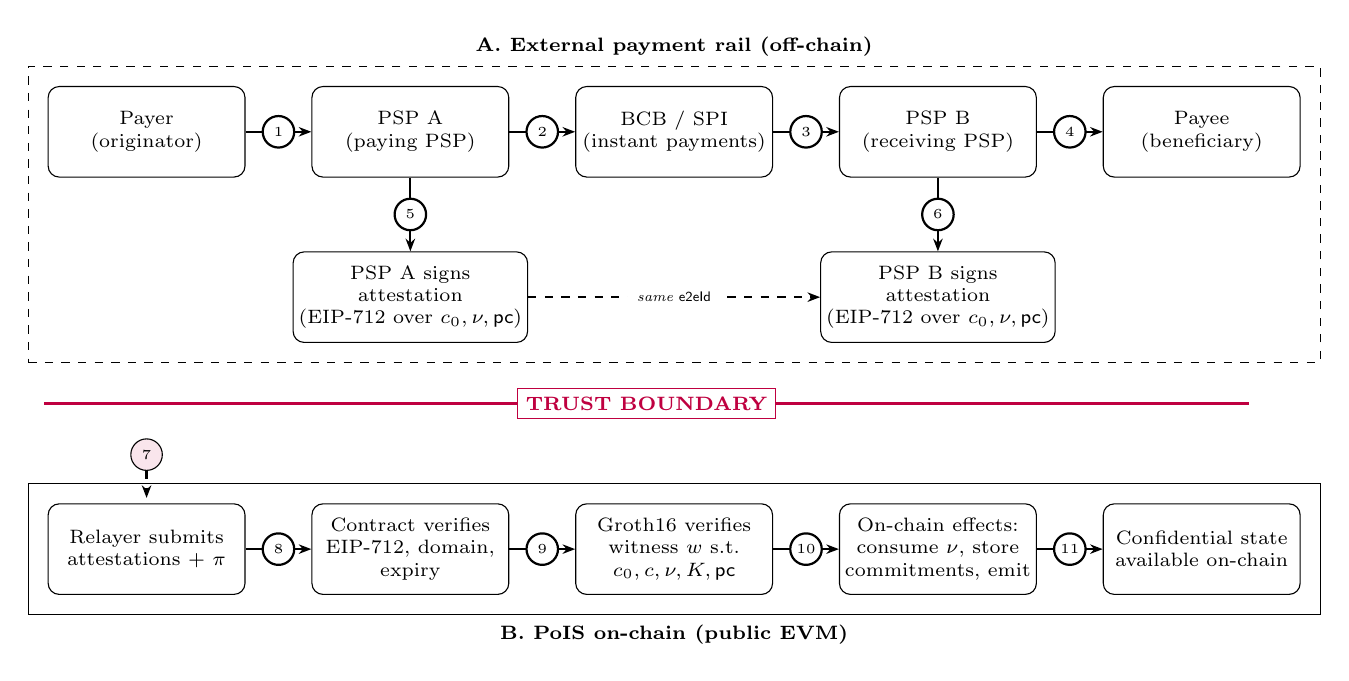
\begin{tikzpicture}[
  box/.style={draw, rounded corners, align=center, minimum height=1.15cm, minimum width=2.5cm, inner sep=2pt, font=\scriptsize},
  stepdot/.style={circle, draw, fill=white, inner sep=0pt, minimum size=4mm, font=\tiny},
  arr/.style={-{Stealth[length=1.6mm]}, thick},
]

  \node[box] (payer)  at (0,4.3)    {Payer\\(originator)};
  \node[box] (pspa)   at (3.35,4.3)  {PSP A\\(paying PSP)};
  \node[box] (spi)    at (6.7,4.3)  {BCB / SPI\\(instant payments)};
  \node[box] (pspb)   at (10.05,4.3) {PSP B\\(receiving PSP)};
  \node[box] (payee)  at (13.4,4.3) {Payee\\(beneficiary)};

  \draw[arr] (payer) -- (pspa)  node[stepdot, midway]{1};
  \draw[arr] (pspa)  -- (spi)   node[stepdot, midway]{2};
  \draw[arr] (spi)   -- (pspb)  node[stepdot, midway]{3};
  \draw[arr] (pspb)  -- (payee) node[stepdot, midway]{4};

  \node[box, minimum width=2.7cm] (attesta) at (3.35,2.2) {PSP A signs\\attestation\\(EIP-712 over $c_0,\nu,\mathsf{pc}$)};
  \node[box, minimum width=2.7cm] (attestb) at (10.05,2.2) {PSP B signs\\attestation\\(EIP-712 over $c_0,\nu,\mathsf{pc}$)};
  \draw[arr] (pspa) -- node[stepdot, midway]{5} (attesta);
  \draw[arr] (pspb) -- node[stepdot, midway]{6} (attestb);
  \draw[arr, dashed] (attesta) -- node[fill=white, midway, font=\tiny\itshape]{same \eeid{}} (attestb);

  \begin{scope}[on background layer]
    \node[draw, dashed, fit=(payer)(pspa)(spi)(pspb)(payee)(attesta)(attestb), inner sep=7pt, label={[font=\bfseries\scriptsize]above:A. External payment rail (off-chain)}] (offchain) {};
  \end{scope}

  \draw[very thick, purple] (-1.3,0.85) -- (14.0,0.85);
  \node[fill=white, draw=purple, inner sep=3pt, font=\bfseries\scriptsize, text=purple] at (6.35,0.85) {TRUST BOUNDARY};

  \node[stepdot, fill=purple!10] (s7) at (0,0.2) {7};
  \draw[arr, dashed] (s7) -- (0,-0.35);
  \node[box] (relayer) at (0,-1.0)   {Relayer submits\\attestations $+\ \pi$};
  \node[box] (verify)  at (3.35,-1.0) {Contract verifies\\EIP-712, domain,\\expiry};
  \node[box] (groth)   at (6.7,-1.0) {Groth16 verifies\\witness $w$ s.t.\\$c_0,c,\nu,K,\mathsf{pc}$};
  \node[box] (effects) at (10.05,-1.0) {On-chain effects:\\consume $\nu$, store\\commitments, emit};
  \node[box] (conf)    at (13.4,-1.0){Confidential state\\available on-chain};

  \draw[arr] (relayer) -- node[stepdot, midway]{8} (verify);
  \draw[arr] (verify)  -- node[stepdot, midway]{9} (groth);
  \draw[arr] (groth)   -- node[stepdot, midway]{10} (effects);
  \draw[arr] (effects) -- node[stepdot, midway]{11} (conf);

  \begin{scope}[on background layer]
    \node[draw, fit=(relayer)(verify)(groth)(effects)(conf), inner sep=7pt, label={[font=\bfseries\scriptsize]below:B. PoIS on-chain (public EVM)}] (onchain) {};
  \end{scope}
\end{tikzpicture}
\caption{PoIS protocol flow. \textbf{A (off-chain)}: (1) the payer initiates a
Pix payment; (2)--(4) the rail carries it through both PSPs to the payee; (5,
6) each PSP that needs to sign attests what it observed, over the
commitments --- never the plaintext value or identifiers. \textbf{Trust
boundary}: everything above is off-chain and PSP-attested; everything below
is on-chain and cryptographically checked --- the off-chain payment event
reaches the on-chain state only through the PSP attestation and the ZK
consistency checks of \S\ref{sec:construction}--\S\ref{sec:oracle}.
\textbf{B (on-chain)}: (7, 8) a relayer submits the attestation(s) and the
Groth16 proof $\pi$; (9) the contract checks the EIP-712 signature, domain
anchor and expiry; (10) the proof is verified; (11) the tag is consumed and
confidential commitments are recorded. This is a schematic of the flow
described in \S\ref{sec:construction}--\S\ref{sec:oracle}; the reference
implementation's negative cases (\S\ref{sec:impl}) exercise each check in box
B individually.}
\label{fig:protocol-flow}
\end{figure}

\section{Preliminaries}

\paragraph{Instant payment / E2EID.} The \code{EndToEndId} is the unique
identifier that accompanies an instant-payment transaction end to end. It is
worth being precise about its provenance, because the design depends on it: the
E2EID is generated \emph{by the payer's PSP at initiation} --- the institution
code (ISPB) embedded in it is the \emph{payer's} --- and it exists for
transactions that are subsequently \emph{rejected} as well as for those that
settle. The central-bank infrastructure (SPI) validates its uniqueness; it does
not mint it. The consequence is the premise of this work:
\emph{possession of an E2EID does not imply settlement}. An identifier alone is a
claim, not a fact, which is precisely why the attestation oracle of
\S\ref{sec:oracle} exists.

\paragraph{Field encoding and canonicalization.} Strings (the E2EID, the PSP
charge id \code{txid}) are mapped to elements of the BN254 scalar field $\Fp$
off-chain via $\mathsf{stringToField}(s) = \mathsf{keccak256}(s) \bmod p$. The
hash is taken over the \emph{exact bytes returned by the PSP API}: UTF-8, with no
case-folding, no trimming, and no re-serialization. This is not a detail --- the
PSP and the institution must hash byte-identical inputs or the attestation and
the proof will refer to different field elements and the settlement will simply
fail to close. Implementations must therefore treat the API response bytes, not a
parsed-and-reprinted string, as the canonical input.

The counterparty identifier committed in $\mathsf{pc}$ (\S\ref{sec:construction})
needs its own canonicalization rule, $\mathsf{CanonicalID}_{\text{rail}}$, and
that rule is necessarily \emph{per-rail}: neither the on-chain contracts nor
the circuits parse an identifier format --- to them $\mathsf{pc}$ is an opaque
field element, and any national ID / instant-payment rail (a US EIN over
FedNow, an IBAN over SEPA Instant, and so on) plugs in by fixing its own
$\mathsf{CanonicalID}_{\text{rail}}$ and computing $\mathsf{pc}$ the same way
on both sides. The PSP and the institution must apply the identical rule:
two formattings of the same identifier are two different field elements, and
$\mathsf{pc}$ computed by one party will not match $\mathsf{pc}$ committed by
the other. Appendix~\ref{app:pix} gives $\mathsf{CanonicalID}_{\text{Pix}}$,
the concrete rule this prototype and its pilot deployment use, kept out of the
core protocol description deliberately: the construction is rail-agnostic, and
a rule specific to Brazilian identifier formats has no place fixing what the
core protocol requires elsewhere. Amounts, finally, are committed as the
integer number of the settlement currency's smallest unit, parsed exactly from
the API's decimal string --- no rounding and no locale formatting --- and the
PSP recomputing $c_0$ must use that same integer: a value-consistency check
that compares two encodings of the same amount fails closed, which is safe but
useless.

\paragraph{Poseidon.} A ZK-friendly hash over $\Fp$; we use the circomlib
instantiations of arity $1$ to $4$~\cite{poseidon}.

\paragraph{Groth16.} A pairing-based zk-SNARK with constant-size proofs (8 field
elements over BN254, $\approx 256$ bytes) and cheap on-chain verification via the
EVM \code{alt\_bn128} precompiles (EIP-196/197)~\cite{groth16}. Groth16 requires
a per-circuit trusted setup; see \S\ref{sec:security} for our stance on it.

\section{Construction}
\label{sec:construction}

\subsection{Two-phase commitment}
A single commitment $c=\Poseidon(\text{amount},\text{salt},\eeid,\text{txid})$,
registered once at settlement, would be the simplest design, but it is only
computable \emph{after} the payment, because the E2EID is born there. The
consequence is structural: at the moment the parties agree on terms there would
be nothing on-chain that an asset escrow can lock onto, and the asset leg
therefore could not be conditioned on the payment leg --- which is exactly what
a delivery-versus-payment composition needs. We therefore split the commitment
in two.

At \textbf{charge creation}, before any payment exists, the orchestrator registers
\begin{equation}
c_0 = \Poseidon(\text{amount}, \text{salt}_0, \text{txid}),
\end{equation}
the commitment to the \emph{agreed terms}. The escrow locks on $c_0$. At
\textbf{settlement}, once the payment has happened, the orchestrator registers
\begin{equation}
c = \Poseidon(\text{amount}, \text{salt}, \eeid, \text{txid}).
\end{equation}
The circuit proves that the \emph{same} amount and the \emph{same} \code{txid}
appear in both, which is what ties the settled payment to the terms that were
agreed before it existed. Nothing in the clear goes on-chain at either phase.
The blinding factors $\text{salt}_0$ and $\text{salt}_p$ are shared with the PSP
at charge creation --- and only these two, never $\text{salt}$ --- so that the PSP
can recompute $c_0$ from the amount it actually settled, and $\mathsf{pc}$ from the
debtor identifier in the payment message (\S\ref{sec:oracle}).

\subsection{Circuit \code{settlement\_verify\_v2}}
\begin{itemize}
\item \textbf{Public signals, in this fixed order:} $c_0$, $c$, the settlement
tag $\nu$, the domain-key anchor $K$, and the counterparty commitment
$\mathsf{pc}$ --- i.e. \code{pubSignals[0..4]}. \code{SettlementV2.finalize}
indexes this array positionally (\S\ref{sec:construction}); the order is fixed
by the circuit's public-signal declaration and cross-checked manually against
the contract's indexing, since \code{verifyProof} itself only checks that the
proof is valid \emph{for the signals as given} --- it enforces nothing about
what a given position is supposed to mean, which is a property the calling
contract, not the verifier, is responsible for getting right.
\item \textbf{Private signals:} amount, $\text{salt}_0$, salt, \eeid, txid, the
domain key $k$, the counterparty \emph{party}, and $\text{salt}_p$.
\item \textbf{Constraints:}
\begin{align}
c_0 &\;\overset{!}{=}\; \Poseidon(\text{amount}, \text{salt}_0, \text{txid}) \\
c   &\;\overset{!}{=}\; \Poseidon(\text{amount}, \text{salt}, \eeid, \text{txid}) \\
\nu &\;\overset{!}{=}\; \Poseidon(\eeid, k) \\
K   &\;\overset{!}{=}\; \Poseidon(k) \\
\mathsf{pc} &\;\overset{!}{=}\; \Poseidon(\text{party}, \text{salt}_p)
\end{align}
\end{itemize}
Equations (3) and (4) share the private witness \emph{amount} and \emph{txid},
which is the two-phase binding. Binding \code{txid} into both commitments prevents
a valid proof for one $(\text{amount}, \eeid)$ from being reused for a different
charge. The settlement circuit places no range constraint on \emph{amount};
well-formedness of the value comes from the PSP recomputing $c_0$ from the
amount it actually settled (\S\ref{sec:oracle}), not from the circuit, and only
the compliance predicate of \S\ref{sec:predicates} decomposes the amount into
bits.

\paragraph{Settlement tag: one symbol, keyed.}
We use a single symbol $\nu$ throughout for the settlement tag --- in ZK
terminology, $\nu$ is a \emph{domain-scoped nullifier}: deterministic in \eeid{}
within a fixed domain key $k$, and recorded as spent on first acceptance, but
(as Property~\ref{prop:uniqueness}, \S\ref{sec:formal}, states precisely) not a nullifier over a
global namespace. We keep ``tag'' as the primary term in the prose that
follows because it is what the reference implementation names it, and flag the
correspondence here once rather than throughout. The unkeyed
variant $\Poseidon(\eeid)$ is not part of the construction (it is retained only
as an ablation row in \S\ref{sec:impl}, to make the keying's cost and necessity
legible). The tag, together with the on-chain registry that records each
accepted value as spent, enforces \emph{single use}: a settled payment closes at
most one operation. $\nu$ itself must be \emph{deterministic} in
\eeid{} --- otherwise the same payment could be replayed under a fresh tag ---
yet not leak \eeid. The na\"ive $\Poseidon(\eeid)$ meets determinism but not
hiding: the E2EID is structured and low-entropy,
\code{E<ISPB:8><timestamp:minute><random>}. The cheap attack is not brute force
over the random suffix; it is \emph{linkage by a party that already holds the
E2EID legitimately}. The payer's own bank, which is not a party to the on-chain
operation, knows the E2EIDs it issued and can simply hash them and look for a
match. We therefore key the tag: $\nu=\Poseidon(\eeid, k)$ with $k$ a domain
secret carrying $\approx 254$ bits (finding RT-5 of our own red team).

\paragraph{Anchoring the domain key.}
A keyed tag raises the question of who holds $k$. If $k$ lives only with the
participants and the PSP, the PSP becomes its custodian and uniqueness holds only
under the informal premise that everyone in a domain used the same key. We
therefore register $K=\Poseidon(k)$ on-chain at domain setup and expose it as a
public signal of the circuit. Two tags accepted under the same $K$ provably come
from the same $k$, so \emph{intra-domain} uniqueness holds by construction rather
than by convention. Cross-domain uniqueness is a different claim and rests on the
PSP's \eeid{}$\to$\code{txid} bijection (Assumption~(I1)).

\paragraph{$\nu$ is a selective-linkability primitive, not a privacy primitive
against the key holder.} Whoever holds $k$ --- the PSP, in this deployment ---
can compute $\Poseidon(\eeid,k)$ for any \eeid{} it observes and therefore map
every $\nu$ in the domain back to the E2EID that produced it: the entire
domain's on-chain tag history is linkable, by construction, to whoever holds
$k$. This is not an oversight to be fixed; it is what makes $k$ do useful work
at all, and it is the same holder as the one already trusted for attestation
(Assumption~(I1)) --- keying $\nu$ adds no new party who can
deanonymize the domain. What the key achieves is narrower and precisely
stated: \emph{public unlinkability for any observer without $k$}, against the
concrete attack of \S\ref{sec:construction} (a party that already holds
E2EIDs legitimately hashing them to find a match) --- combined with
\emph{intentional, domain-scoped linkability for whoever holds $k$}. Calling
this ``privacy'' without the second half would overstate it.

\paragraph{Key rotation.}
The anchor makes $K$ immutable for the lifetime of a domain, and this is
deliberate: if a domain rotated $k$ to $k'$, the same \eeid{} would produce a
fresh tag $\nu'=\Poseidon(\eeid,k')$, and the tag registry --- which by design
cannot see \eeid{} --- would accept a second settlement of an already-settled
payment. Rotation is therefore expressed as starting a \emph{new} domain (new
$K$, new escrows), and uniqueness across the two domains is not enforced by the
circuit: like cross-domain uniqueness in general, it rests on the PSP's
\eeid{}$\to$\code{txid} bijection (Assumption~(I1)). A deployment that
anticipates key compromise should treat this as an operational cost of the
design, not a footnote. Put precisely: \emph{domain separation is a security
boundary}, the thing uniqueness (Property~\ref{prop:uniqueness}) is stated
relative to, not merely a key-management convenience --- crossing it is
exactly where the unconditional guarantee ends and Assumption~(I1)
begins.

\paragraph{Counterparty commitment.}
The compliance predicates of \S\ref{sec:predicates} speak about a counterparty.
For them to mean anything, that counterparty must be the one that actually paid.
We therefore make $\mathsf{pc}=\Poseidon(\text{party},\text{salt}_p)$ a public
signal of the settlement circuit \textbf{and} a signed field of the PSP receipt
(\S\ref{sec:oracle}): the PSP computes $\mathsf{pc}$ over the debtor identifier
(CPF/CNPJ) exactly as it appears in the payment message, canonicalized per
\S\ref{sec:construction} above, using the $\text{salt}_p$ shared at charge
creation, and \code{finalize} accepts only if the attested $\mathsf{pc}$ equals
the proof's public signal. For charges that do not pin a debtor at creation, the
PSP computes $\mathsf{pc}$ at attestation time, when the payment message names the
payer. Without both halves the predicates are decorative --- the prover picks the
party; with them, the counterparty the predicates speak about is, by
construction, the counterparty that paid. We return to this in
\S\ref{sec:predicates}.

\subsection{Protocol}
\begin{enumerate}
\item The receiving institution creates a \emph{real} instant-payment charge through a PSP
(e.g. a PSP sandbox), obtaining a \code{txid}. The commitment $c_0$ to the agreed
terms is registered on-chain and the asset escrow locks on it.
\item The charge (the instant-payment payload string and \code{txid}) is exchanged
\emph{encrypted, peer-to-peer and off-chain} between the two institutions, with
an optional on-chain anchor of its hash. It is deliberately \emph{not} written
encrypted to the chain: a ciphertext over a payment key, a value and a charge
identifier, recorded permanently on a public ledger, is a harvest-now-decrypt-later
target that the post-quantum channel of \S\ref{sec:pq} protects for auditor
disclosure but would not protect here, and it is personal data written to an
immutable medium, which is a poor posture under the Brazilian data-protection law.
\item The paying institution makes the instant payment; the PSP confirms; the
\code{E2EID} is resolved.
\item The PSP signs an EIP-712 receipt over $(c_0,\nu,\mathsf{pc},\mathsf{settled},
\mathsf{deadline})$, recomputing $c_0$ from the amount it settled and
$\mathsf{pc}$ from the debtor identifier in the payment message; the oracle
attests it (\S\ref{sec:oracle}).
\item The proof $\pi$ is generated over the public signals $(c_0,c,\nu,K,\mathsf{pc})$
and \code{finalize}$(\pi)$ requires the operation to be \textsc{Locked} and
$\nu$ unused, checks the domain anchor $K$, cross-checks the oracle attestation
for $\nu$ (same $c_0$ and same $\mathsf{pc}$), then verifies $\pi$, and only
then consumes the tag and transitions the operation to \textsc{Finalized}; the
cheap checks run before the pairing so that a mismatched receipt reverts
without paying for verification. It becomes
\textsc{Irrevocable} only after the rail's refund window elapses without a
reversal (\S\ref{sec:oracle}).
\end{enumerate}

\section{The Attestation Oracle}
\label{sec:oracle}

The circuit proves \emph{knowledge} of a preimage; it does \emph{not}, on its
own, prove that the E2EID corresponds to a payment actually settled at the SPI.
Historically this was resolved purely off-chain: the PSP confirms the payment,
returns the E2EID, and the paying institution submits it --- an unverified claim.
As \S2 notes, an E2EID exists for rejected payments too, so the claim is not even
self-evidencing.

\subsection{A receipt that does not carry the value}
The oracle makes the trust link explicit and on-chain verifiable. A trusted PSP
(the \emph{attestor}) signs, off-chain, an EIP-712 receipt
\[
\mathsf{Receipt}(\underbrace{c_0}_{\text{bytes32}},\;
\underbrace{\nu}_{\text{settlement tag}},\;
\underbrace{\mathsf{pc}}_{\text{counterparty commitment}},\;
\underbrace{\mathsf{settled}}_{\text{bool}},\;
\underbrace{\mathsf{deadline}}_{\text{uint64}}),
\]
and any relayer submits it via \code{attest(receipt, signature)}.

The choice of fields matters because the naive alternative genuinely leaks.
Consider signing
$\mathsf{Receipt}(\text{txid},\nu,\text{amount},\mathsf{settled})$ instead: since
the contract must recompute the EIP-712 digest to recover the signer, every
signed field necessarily appears \emph{in the clear in the calldata} of
\code{attest}, which is public and permanent --- and a naive implementation is
likely to also emit the amount in an event, for indexing. Since $\nu$ is the
same tag the settlement circuit exposes, any observer could join the public
settlement $(c,\nu)$ to that attestation and read off the amount. Such a design
would falsify the confidentiality claim of \S\ref{sec:security} and
Property~\ref{prop:conf}, and the amount would not even be used in any on-chain
check --- pure liability for no benefit.

Signing over $c_0$ avoids the leak and, unlike signing the amount directly,
\emph{adds} a check rather than a mere pass-through. The PSP holds
$\text{salt}_0$ and \code{txid} from charge creation and
observes the amount it actually settled; it recomputes $c_0$ from those three
values. \textbf{This recomputation is normative, not an implementation detail:
the PSP must evaluate the Poseidon itself --- for $c_0$ over the amount it
observed settling, for $\mathsf{pc}$ over the debtor identifier in the payment
message, and for the tag $\nu=\Poseidon(\eeid,k)$ over the E2EID it observed,
using the domain key it holds --- and must never sign a $c_0$, $\mathsf{pc}$ or
$\nu$ value received from the institution.} A PSP whose API merely echoes a
client-supplied commitment turns the value-consistency check into a tautology ---
the signature would attest that the client's number equals the client's number
--- and a client-supplied tag is worse: it would let the institution attach an
arbitrary tag to a real payment, severing the anti-replay binding between $\nu$
and the E2EID, unless the PSP kept its own \eeid{}$\to$attested registry, which is
exactly the state this design avoids. This is the same failure shape as the
vacuous verification verdict of \S\ref{sec:formalver}, one layer up, and an
integration audit should test for it explicitly.

A payment for the wrong amount produces a different $c_0$, the receipt
then refers to a commitment the escrow is not locked on, and the settlement does
not close. The protocol thus verifies \emph{value consistency without the value
appearing anywhere on-chain}. The \code{deadline} bounds the window in which a
signed receipt can be used, containing the damage from a compromised PSP key ---
provided the attestor bounds it: the contract enforces
\code{block.timestamp <= deadline} and no upper cap, so a receipt signed with a
distant deadline stays usable until then. The receipt additionally carries
$\mathsf{pc}$, the counterparty commitment of
\S\ref{sec:construction}, which the PSP computes over the debtor identifier in the
payment message using the $\text{salt}_p$ shared at charge creation. This adds
nothing to what an observer sees: $\mathsf{pc}$ is already a public signal of the
settlement proof, it is a Poseidon image under a $\approx 254$-bit salt, and the
attestation and the settlement were already linkable through $\nu$. What it adds
is a check: \code{finalize} accepts only if the attested $\mathsf{pc}$ equals the
proof's public signal, so the counterparty the compliance predicates speak about
is the one the PSP saw paying --- not one the prover chose.

The contract recovers the signer with \code{ECDSA.recover} over the EIP-712 digest
and accepts \emph{iff}: the signer is a registered attestor; $\mathsf{settled}
=\textsf{true}$; the receipt has not expired; and $\nu$ has never been attested
(anti-replay). On success it records $(\nu \mapsto \text{signer}, c_0,
\mathsf{pc}, \text{timestamp})$ --- in the reference implementation $c_0$ and
$\mathsf{pc}$ are stored as the single word
$\mathsf{keccak256}(c_0 \Vert \mathsf{pc})$, which keeps the storage footprint of
the attestation unchanged --- and emits an event that carries \emph{no} amount, no
charge identifier and no party identifier. The PSP is gasless: it only signs; the
relayer pays gas and holds no power to forge, since acceptance is gated on the PSP
signature.

Two consequences of sharing the blinding factors deserve stating. Against the PSP
itself, $c_0$ and $\mathsf{pc}$ are not hiding at all --- by design: the check is
the PSP recomputing them, and since the PSP separately holds every other
preimage it processed (amount, \code{txid}, \eeid, party, and the salts), it is,
by construction, a complete linkability oracle for the operations that pass
through it: nothing in this protocol hides the fiat leg from the PSP that
services it (\S\ref{sec:security} states this as a scope boundary of the
confidentiality claim, not an oversight). Against any third party that obtains
$\text{salt}_0$ (or
$\text{salt}_p$), the hiding of $c_0$ (or $\mathsf{pc}$) degrades from the salt's
$\approx 254$ bits to the entropy of the remaining preimage: for $\mathsf{pc}$ that
is the CPF/CNPJ space, enumerable outright; for $c_0$ it is $(\text{amount},
\text{txid})$, enumerable only if the charge id --- $26$ to $35$ alphanumeric
characters --- leaks through the same channel, which in practice it does. The
salts are therefore secrets of the same sensitivity as the payment data they
blind, and the off-chain channel of \S\ref{sec:construction} step~2 must protect
them accordingly. And since \code{attest} is write-once per tag, a receipt the PSP
signs over a \emph{wrong} recomputed $c_0$ --- a software bug, not an attack ---
permanently burns that $\nu$: the payment can no longer close \emph{that}
operation, and the $c_0$ it was locked on falls back on the liveness timeout
of \S\ref{sec:oracle} (\code{cancel}, once the \code{lock} deadline passes)
rather than staying stuck. We state this as a property of the anti-replay
choice rather than discover it in production.

\subsection{What \texttt{settled} means, and reversal}
\label{sec:reversal}
Settlement at the SPI is not the end of the story. The rail provides a return
mechanism (certain Pix return/fraud-recovery mechanisms may remain effective for
up to 90 days), a dedicated fraud-refund mechanism, and the receiving PSP may
place a precautionary hold of up to 72 hours. We therefore define, as an
internal semantic of this protocol's \code{settled} field --- not a redefinition
of the rail's own settlement terminology --- that $\mathsf{settled}=\textsf{true}$
means \emph{credit available to the receiver}, not merely ``cleared at the
SPI''; this is what the PSP must observe before it may sign a receipt with
$\mathsf{settled}=\textsf{true}$ (\S\ref{sec:oracle}).

Accordingly the oracle exposes \code{attestReversal}, in which the \emph{same}
attestor signs $(\nu,\mathsf{returned}=\textsf{true},\mathsf{deadline})$ within a
configured dispute window, and the operation state machine distinguishes
\textsc{Finalized} from \textsc{Irrevocable}: the latter is reached only once the
window elapses with no reversal. \textbf{Read \textsc{Irrevocable} as a
protocol-state name, not an economic-finality claim}: it means only that
\emph{this contract} will no longer accept a reversal for this operation ---
which, as the very next paragraph quantifies, is not the same as the rail
being unable to reverse the underlying payment for the following $\approx 87$
days. A delivery-versus-payment flow must gate the
irreversible release of the asset on \code{isIrrevocable}, not on
\code{isAttested}, while still pricing in that residual rail-level risk
separately. Revoking an attestor blocks \emph{new} attestations and does
not retroactively invalidate past ones; retroactive invalidation would hand the
registry owner the power to undo completed settlements.

The state machine is deliberately open to one orthogonal upgrade: a
\code{RailAnchored} flag, settable at any time by a verified rail-level statement
(\S\ref{sec:security}, path~iv), which strengthens the evidence behind a
\textsc{Finalized} or \textsc{Irrevocable} operation --- and, applied to returns,
narrows the post-window residual above from invisible to visible ex post ---
without ever sitting on the settlement's critical path.

One trade-off must be stated numerically rather than implied. The dispute window
is a deployment parameter, and the reference deployment sets it to $72$ hours.
That figure mirrors the rail's precautionary-hold period, but under the
credit-available semantics above it corresponds to \emph{no} rail deadline: a hold
is resolved before the PSP attests, and the mechanisms that can still reverse a
credited payment --- the ordinary return, which may remain effective for up to
$90$ days, and the dedicated fraud-refund mechanism, on its own separate track
--- extend far beyond it. The $72$-hour window therefore
catches early returns only. An operation that reaches \textsc{Irrevocable} after
$72$ hours remains exposed, for the remaining $\approx 87$ days, to a rail-level
refund that the on-chain state machine will not represent; that residual risk sits
with the asset leg, and a deployment accepts it as the price of not locking
capital for three months. A deployment that instead requires \textsc{Irrevocable}
to dominate the refund window must set the window to $90$ days and carry the
capital cost. Both are defensible; choosing silently is not, so the reference
artifacts choose $72$ hours and say so.

\section{Confidential Compliance Predicates}
\label{sec:predicates}

Beyond proving that fiat settled, a regulated deployment must answer
questions about a transaction \emph{without opening it}. We extend the commitment
scheme with three ZK \emph{policy predicates}, each a small Groth16 circuit
whose only public signals are commitments and a policy anchor; the sensitive
data never appears, \emph{not even to the auditor}. We call them policy
predicates rather than compliance predicates deliberately: each proves
membership or a bound against an on-chain policy anchor set by a named
authority (\S\ref{sec:predicates}, ``Policy authority on-chain''), which is
necessary input to a compliance determination but does not itself constitute
one --- amount-within-limit is a policy condition, not a legal category, and
the two membership predicates below are named to make the same point
explicit.

\begin{itemize}
\item \textbf{Value within limit} (\code{compliance\_range\_verify}): proves
$\text{amount} < \text{limit}$ for an opening of the commitment, via a bounded
comparison ($\code{Num2Bits}(64)$ range-checking both operands, then
\code{LessThan}).
\item \textbf{Non-membership in the attested sanctions set}
(\code{sanctions\_exclusion\_verify}): proves the counterparty, committed as
$\mathsf{pc}$, is \emph{absent} from a Sparse Merkle Tree of sanctioned parties
(circomlib \code{SMTVerifier} non-membership, $\code{fnc}=1$). We name it this
way, not ``sanctions clearance'', deliberately: the predicate proves absence
from \emph{the specific set the anchored root represents}, at the root's
version, under whatever normalization built it (\S\ref{sec:predicates},
Open operational questions, item~i) --- it is not equivalent to a legal
determination that the counterparty is unsanctioned, which depends on list
freshness, normalization and coverage the circuit has no visibility into.
\item \textbf{KYC-set membership} (\code{kyc\_inclusion\_verify}): the mirror
predicate --- proves the counterparty is \emph{present} in an allow-list SMT of
identities the root's operator has verified ($\code{fnc}=0$). Likewise not
``KYC compliance'': that determination is delegated entirely to whichever
authority admits identities into the root and governs its lifecycle (who
verified, when, under what jurisdiction, whether revoked) --- the predicate
proves set membership, nothing about the verification behind it.
\end{itemize}

\paragraph{Whose counterparty?}
A predicate about a party the prover chose is worthless. If the counterparty
commitment were an independent input to each predicate circuit, a malicious
institution could commit to any clean identity and prove exclusion and inclusion
about \emph{that} identity while settling a payment involving someone else ---
with no counterparty field on the settlement side to contradict it. The
construction closes this structurally, with two halves: $\mathsf{pc}$ is a
public signal of the settlement circuit
(\S\ref{sec:construction}), so settlement and predicates provably speak about the
same committed party; and $\mathsf{pc}$ is a signed field of the PSP receipt
(\S\ref{sec:oracle}), computed over the debtor identifier in the payment message,
with \code{finalize} requiring equality between the attested value and the
proof's public signal. The predicates consume that same $\mathsf{pc}$. The
counterparty they speak about is then, by construction, the counterparty that
paid --- under Assumption~(I1): a PSP that signs a wrong $\mathsf{pc}$ is
the same trusted-PSP residue as a PSP that signs a false $\mathsf{settled}$.

\paragraph{Policy authority on-chain.}
The policy anchor (the \code{limit}, or the \code{sanctionsRoot}/\code{kycRoot})
must be fixed by an on-chain policy authority, not supplied by the prover.
Otherwise a malicious institution could prove compliance against a favorable
self-chosen limit, or exclusion against an empty sanctions tree. The attestors
pin the official policy (\code{setPolicyLimit}/\code{setKycRoot}, guarded by a
\code{policyAdmin}) and reject any proof whose public policy signal does not equal
it. We validated, in the reference repository's compliance demonstration on
the same testnet (whose transactions are not part of the artifact manifest of
\S\ref{sec:impl}), that a \emph{genuinely valid} Groth16 proof for a
self-chosen loose limit is rejected precisely because it does not match the
official policy.

\paragraph{Open operational questions.}
We flag three that the cryptography does not settle and a deployment must.
\emph{(i) List normalization}: sanctions lists are keyed differently ---
OFAC matches on names and aliases, the Brazilian CEIS/CNEP registries on
CPF/CNPJ. An SMT over identifiers cannot express name-matching semantics, so a
deployment must fix a normalization and accept the resulting false-negative
profile explicitly. \emph{(ii) Root lifecycle}: who updates \code{sanctionsRoot},
how often, and --- the sharp question --- whether proofs issued against a
superseded root remain valid. Both answers are defensible; leaving it implicit is
not. \emph{(iii) Per-transaction limit is not AML}: the range predicate bounds a
single transaction and says nothing about structuring across many. Aggregate
monitoring is a different problem and we do not claim to address it.
\emph{(iv) Whose identity, precisely}: naming this precisely matters more than
it looks, so we fix three terms rather than use ``counterparty'' loosely.
$\mathsf{payerId}$ is the debtor account holder exactly as named in the
payment message --- what $\mathsf{pc}$ actually commits. The
\emph{economicCounterpartyId} is whoever the transaction is economically
for, which coincides with $\mathsf{payerId}$ except when a third party pays on
the debtor's behalf. The \emph{beneficialOwnerId} is a further AML/KYC concept
(who ultimately controls or benefits, e.g. behind a shell entity) that this
construction does not represent at all. Precisely stated, then: the policy
predicates of this section prove a predicate about $\mathsf{payerId}$, always;
a deployment must decide whether third-party payments are rejected at
attestation (so $\mathsf{payerId}=\mathsf{economicCounterpartyId}$ always
holds), or accepted with $\mathsf{pc}$ understood as ``who actually paid'' ---
the more defensible question for AML purposes, but a different question from
``who is the beneficial owner'', which this construction leaves entirely to
the PSP's own KYC process and does not attempt to answer.

\section{Post-Quantum Audit Disclosure: A Preliminary Construction}
\label{sec:pq}

\noindent\emph{This section is an optional, crypto-agile audit-disclosure
channel and is not part of the core Proof-of-Instant-Settlement security
argument} (\S\ref{sec:formal}--\S\ref{sec:security}): none of the properties
or the threat-model rows there depend on anything in this section, and a
deployment can run the settlement construction with only the classical
(X25519) channel selected. We report it here as a preliminary, sized
construction, not as a claim the core contribution rests on.

Auditor disclosure has \emph{long-lived} confidentiality: a ciphertext recorded
today must resist a future quantum adversary (``harvest now, decrypt later''). The
disclosure channel is therefore crypto-agile and selectable per deployment ---
classical (X25519), post-quantum (ML-KEM-768, FIPS-203~\cite{mlkem}), or a hybrid
of the two --- declared on-chain (\code{auditChannelKind}, default hybrid) and, in
the intended deployment, changeable only through consortium governance (a
timelocked proposal, not an administrator setter). The reference artifacts, being
a single-maintainer prototype, stand a single admin key in for that governance ---
the same honesty caveat as the registry owner in \S\ref{sec:security} --- so the
governance property should be read as \emph{designed}, not as \emph{demonstrated}.
Each auditor publishes its own encryption key, so no administrator can redirect it
to intercept disclosures.

\paragraph{In-circuit binding.}
To make a disclosure \emph{verifiable by anyone without decrypting}, we prove in
zero knowledge that the published ciphertext encrypts the opening of the
commitment under a key derived from the KEM shared secret. Following
Qurrency~\cite{qurrency} --- which uses the \emph{same} Groth16/circom/Poseidon
/BN254 stack --- we port its open-source (Apache-2.0) ML-KEM-in-circom
implementation and connect \code{mlkem\_encaps} to our commitment. The resulting
circuit \code{audit\_binding\_pq\_verify} compiles at $\approx 1.62$M constraints;
the shared secret is thereby \emph{proven} to originate from ML-KEM, not merely
asserted. A symmetric-only binding (shared secret as a private input) is validated
on-chain in the interim; the trusted-setup ceremony for the full
$1.62$M-constraint circuit requires production hardware ($\sim 16$\,GB RAM,
$2^{21}$ powers of tau) and is deferred to the pilot.

\paragraph{Status (preliminary).}
We report this post-quantum binding as \emph{preliminary}. Unlike the settlement
circuits --- for which we give proving time and on-chain verification gas ---
the full in-circuit ML-KEM binding has no end-to-end
proving-time or on-chain figure yet, pending the production-scale setup. What is
established is that it \emph{compiles and is sized} on our exact stack; the
selectable channel and the symmetric binding are validated; the full binding is
work in progress rather than a deployed result.

\section{Formal Model and Security Properties}
\label{sec:formal}

We give a syntax for the construction and state its security properties under
explicit cryptographic, operational, institutional and governance assumptions
--- the table below (A1)--(A4) names which assumption is which kind; not
every property that follows reduces to a standard cryptographic assumption
alone, and we say so at each one rather than let ``formal properties'' imply
otherwise. Let $\Pi=(\mathsf{Setup},\mathsf{Commit},\mathsf{Prove},
\mathsf{Verify},\mathsf{Attest},\mathsf{Settle})$ over the BN254 scalar field $\Fp$:
\begin{itemize}
\item $\mathsf{SetupZK}(1^\lambda)\to(\mathsf{crs},\mathsf{vk})$: the per-circuit
Groth16 common reference string and verification key.
\item $\mathsf{SetupDomain}(1^\lambda)\to(k,K)$: a fresh domain key $k$ and its
on-chain anchor $K=\Poseidon(k)$, registered at domain creation and immutable
thereafter (\S\ref{sec:construction}). The two setups are independent: a domain
can be created without a new ceremony, and the ceremony says nothing about any
domain's key.
\item $\mathsf{Commit}_0(\text{amount},\text{salt}_0,\text{txid})\to c_0$ and
$\mathsf{Commit}(\text{amount},\text{salt},\eeid,\text{txid})\to c$.
\item $\mathsf{Prove}(\mathsf{crs},w)\to(\pi,\nu)$ with witness $w=(\text{amount},
\text{salt}_0,\text{salt},\eeid,\text{txid},k,\text{party},\text{salt}_p)$ and
tag $\nu=\Poseidon(\eeid,k)$.
\item $\mathsf{Verify}(\mathsf{vk},c_0,c,\nu,K,\mathsf{pc},\pi)\to\{0,1\}$.
\item $\mathsf{Attest}$: a registered PSP signs (EIP-712) a receipt
$\mathsf{Receipt}(c_0,\nu,\mathsf{pc},\mathsf{true},\mathsf{deadline})$,
recomputing $c_0$ and $\mathsf{pc}$ itself (\S\ref{sec:oracle}).
\item $\mathsf{Settle}$: accept iff $\mathsf{Verify}=1$, the receipt signature
verifies against a registered attestor, the receipt is unexpired, its $c_0$ is the
one the escrow locked on, its $\mathsf{pc}$ equals the proof's public counterparty
commitment, and the tag is unused.
\end{itemize}
We assume: \textbf{(A1)} Groth16 is knowledge-sound and zero-knowledge under its
trusted setup~\cite{groth16}; \textbf{(A2)} $\Poseidon$ is collision-resistant
and, on an input with a high-entropy component, hiding (modeled as a random
oracle)~\cite{poseidon}; \textbf{(A3)} ECDSA/EIP-712 is EUF-CMA; \textbf{(A4)}
within a domain, \code{txid} uniquely identifies the agreed payment obligation
and is not legitimately reused for two distinct charges (Charge-identifier
uniqueness); \textbf{(A5)} $\mathsf{keccak256}$ is collision-resistant for the
binding hash the attestation oracle computes over $(c_0,\mathsf{pc})$
(\S\ref{sec:oracle}). (A4) is what lets \code{txid} do the anti-cross-charge work
Equations (3)--(4) rely on (\S\ref{sec:construction}); it is imposed
operationally by the charge-creation flow (the orchestrator mints a fresh
\code{txid} per charge and the PSP's own charge API rejects a duplicate), not
proved by the circuit, which only checks that \emph{the same} witness
\code{txid} appears in both commitments. (A5) is stated separately from (A2)
because the two hash functions are used for different purposes and neither
collision-resistance assumption implies the other: $\Poseidon$ binds
circuit-internal witness values, while $\mathsf{keccak256}$ binds the
oracle's off-circuit $(c_0,\mathsf{pc})$ pair to a single $\nu$
(Theorem~\ref{thm:settlementbinding}). The assumptions above are not all the
same \emph{kind} of assumption, and treating them as if they were is itself a
source of overclaiming:

\begin{center}
\small
\begin{tabular}{@{}lll@{}}
\toprule
\textbf{Assumption} & \textbf{Nature} & \textbf{Failure mode if false} \\
\midrule
(A1) Groth16 sound./ZK & cryptographic & forged proofs / leaked witness \\
(A2) Poseidon coll.-res. & cryptographic & two openings of one commitment \\
(A2) Poseidon hiding & heuristic (RO model) & preimage recovery, if the model is wrong \\
(A3) ECDSA/EIP-712 EUF-CMA & cryptographic & forged attestations \\
(A4) \code{txid} uniqueness & operational & cross-charge proof reuse \\
(A5) Keccak-256 coll.-res. & cryptographic & oracle binding forged (pc substitution) \\
(I1) Trusted PSP & institutional & false \code{settled} accepted \\
(S1) Trusted setup & cryptographic, contingent on process & forged proofs, if toxic waste leaked \\
Policy-root correctness & governance & wrong predicate answers accepted \\
\bottomrule
\end{tabular}
\end{center}
\noindent The cryptographic rows are the ones a reduction can be stated
against; the operational, institutional and governance rows cannot be
discharged by better cryptography, only by better process, and no amount of
tightening the ZK layer changes that.

\begin{property}[Correctness]
\label{prop:correctness}
For an honestly generated $(c_0,c,\nu,K,\mathsf{pc},\pi)$ of a settled payment
with a valid, unexpired PSP receipt, $\mathsf{Settle}$ accepts.
\end{property}

The next property is stated in three parts on purpose: binding, two-phase
consistency and settlement binding are three different guarantees that a
single ``operation binding'' statement would blur together, and a reviewer
should be able to attack each independently.

\begin{property}[2A --- Commitment binding]
\label{prop:binding}
No PPT adversary produces two distinct openings of the same $c$ (or of $c_0$),
except with negligible probability.
\end{property}
\begin{proof}[Proof sketch]
Two distinct openings of one Poseidon image are a collision, contradicting (A2)
directly; this holds independent of Groth16 or of any protocol logic above it.
\end{proof}

\begin{property}[2B --- Two-phase consistency]
\label{prop:twophase}
For any accepting proof $\pi$ for public inputs $(c_0,c,\nu,K,\mathsf{pc})$,
the amount and \code{txid} used to construct $c$ are identical to those
used to construct $c_0$.
\end{property}

\begin{theorem}[Two-phase consistency]
\label{thm:twophase}
Assuming the knowledge soundness of Groth16 (A1), except with negligible
probability, every accepting proof admits a witness
$w=(\text{amount},\text{salt}_0,\text{salt},\eeid,\text{txid},k,\text{party},
\text{salt}_p)$ satisfying the circuit relation of \S\ref{sec:construction}
(Equations 3--7). In that relation, the same witness values \emph{amount}
and \code{txid} occur in both commitment equations --- Equation~(3),
$c_0=\Poseidon(\text{amount},\text{salt}_0,\text{txid})$, and Equation~(4),
$c=\Poseidon(\text{amount},\text{salt},\eeid,\text{txid})$. Consequently, an
accepting proof cannot represent a transition in which the amount or
\code{txid} used for the post-payment commitment $c$ differs from the
amount or \code{txid} committed at escrow creation, i.e.\ in $c_0$.
\end{theorem}

\begin{proof}
Let $\pi$ be an accepting Groth16 proof. By knowledge soundness (A1), except
with negligible probability, there exists an extracted witness $w$
satisfying the circuit relation. The circuit contains a single witness
variable \emph{amount}, used in both Equation~(3) and Equation~(4), and a
single witness variable \code{txid}, likewise used in both. There are
therefore no independent values $\text{amount}_0,\text{amount}_1$ or
$\text{txid}_0,\text{txid}_1$ that could be chosen separately for $c_0$ and
$c$: the circuit relation does not admit them. Thus, for every accepting
witness, $\text{amount}_{c_0}=\text{amount}_c=\text{amount}$ and
$\text{txid}_{c_0}=\text{txid}_c=\text{txid}$. A proof for which either
value differed between the two phases would require a witness satisfying a
circuit relation the circuit does not define; by knowledge soundness, no
such witness can be extracted from an accepting proof except with negligible
probability. Therefore,
\begin{equation}
\Pr[\mathsf{Bad}_{2B}(\mathcal{A})]
\;\leq\;
\mathrm{Adv}^{\mathrm{KS}}_{\mathrm{Groth16}}(\mathcal{A}),
\end{equation}
where $\mathsf{Bad}_{2B}(\mathcal{A})$ is the event that $\mathcal{A}$
produces an accepting proof whose extracted witness assigns different
amount or \code{txid} values to $c_0$ and $c$.
\end{proof}

\begin{corollary}[Escrow-to-settlement term consistency]
\label{cor:escrowconsistency}
If an escrow is created against $c_0$, any subsequently accepted proof for
that escrow necessarily uses the same amount and \code{txid} in its
post-payment commitment $c$. The property does not by itself establish that
either commitment corresponds to a real-world payment; that semantic fact
remains outside the cryptographic relation and is handled by the PSP
attestation (Property~\ref{prop:auth}) and the Trusted-PSP assumption
(Assumption~(I1)).
\end{corollary}

\begin{property}[2C --- Authenticated settlement binding]
\label{prop:settlementbinding}
Let $D$ be a domain with registered anchor $K_D=\Poseidon(k_D)$, where $k_D$
is the domain secret; elsewhere in this paper, where a single domain is
fixed throughout, we write $K$, $k$ without the subscript, and $K_D$, $k_D$
specialize to exactly those when $D$ is held fixed. Let an adversary
$\mathcal{A}$ interact with the public settlement system and submit
arbitrary proofs and receipts to the attestation oracle and $\mathsf{Settle}$.

An accepted settlement is \emph{authenticatedly settlement-bound} if, except
with negligible probability, there exist a registered attestor $P$; an
EIP-712 receipt $R=(c_0,\nu,\mathsf{pc},\mathrm{true},\mathsf{deadline})$; a
valid PSP signature $\sigma=\mathsf{Sign}_P(R)$; and a Groth16 witness
$w=(\text{amount},\text{salt}_0,\text{salt},\eeid,\text{txid},k,\text{party},
\text{salt}_p)$ satisfying the circuit constraints of \S\ref{sec:construction}
(Equations 3--7), restated here for convenience:
\begin{align*}
c_0 &= \Poseidon(\text{amount},\text{salt}_0,\text{txid}), &
c   &= \Poseidon(\text{amount},\text{salt},\eeid,\text{txid}), \\
\nu &= \Poseidon(\eeid,k), &
K_D &= \Poseidon(k), \\
\mathsf{pc} &= \Poseidon(\text{party},\text{salt}_p), & &
\end{align*}
and, moreover, the receipt authenticated by $P$ is bound to exactly the same
$c_0$, $\nu$, and $\mathsf{pc}$ accepted by $\mathsf{Settle}$.

This property is an authentication and cryptographic-consistency property.
It does \textbf{not} assert that the PSP's statement $\mathsf{settled}=
\mathrm{true}$ is truthful. The latter remains Assumption~(I1).
\end{property}

\begin{theorem}[Settlement-binding theorem]
\label{thm:settlementbinding}
Conditioned on the deterministic correctness of the deployed
$\mathsf{Settle}$ contract with respect to the acceptance conditions
specified in \S\ref{sec:construction} --- a property of the deployed code,
not a cryptographic hypothesis, and hence not itself a term in the bound
below --- and on the registered domain anchor $K_D$ being immutable during
the lifetime of domain $D$ (\S\ref{sec:construction}), assume further: (1)
Groth16 is knowledge-sound for the deployed \code{settlement\_verify\_v2}
circuit; (2) $\Poseidon$ is collision-resistant over the BN254 field; (3)
ECDSA/EIP-712 is EUF-CMA secure; (4) $\mathsf{keccak256}$ is
collision-resistant for the oracle's binding hash --- exactly (A1)--(A3) and
(A5) above, gathered here so the theorem's cryptographic hypotheses are
self-contained rather than scattered.

Then, for every probabilistic polynomial-time adversary $\mathcal{A}$, the
probability that $\mathcal{A}$ causes $\mathsf{Settle}$ to accept a
settlement for which either (a) no registered PSP signed the accepted tuple
$(c_0,\nu,\mathsf{pc},\mathrm{true},\mathsf{deadline})$, or (b) the accepted
$\nu$ is not equal to $\Poseidon(\eeid,k_D)$ for the \eeid{} contained in an
accepting witness for the registered domain, is negligible. More precisely,
\begin{equation}
\Pr[\mathsf{Bad}_{SB}(\mathcal{A})]
\;\leq\;
\mathrm{Adv}^{\mathrm{EUF\text{-}CMA}}_{\mathrm{ECDSA}}(\mathcal{A})
+\mathrm{Adv}^{\mathrm{KS}}_{\mathrm{Groth16}}(\mathcal{A})
+\mathrm{Adv}^{\mathrm{CR}}_{\Poseidon}(\mathcal{A})
+\mathrm{Adv}^{\mathrm{CR}}_{\mathrm{Keccak}}(\mathcal{A}),
\end{equation}
where each term on the right is the standard cryptographic advantage
against the named primitive, and the bound holds under the deterministic
conditioning stated above --- a contract-correctness failure is a software
bug outside the reduction, not a probabilistic event the reduction
accounts for.
\end{theorem}

\noindent The theorem binds $\nu$ to the \eeid{} contained in the accepting ZK
witness; it does \textbf{not}, by itself, establish that the PSP observed
that same \eeid{}. That latter correspondence is part of the Trusted-PSP
assumption (I1).

\begin{proof}
Suppose $\mathcal{A}$ causes $\mathsf{Settle}$ to accept an operation. By the
acceptance condition of $\mathsf{Settle}$, the submitted Groth16 proof
verifies against the public tuple $(c_0,c,\nu,K_D,\mathsf{pc})$. By Groth16
knowledge soundness, except with negligible probability there exists an
extractor obtaining a witness $w=(\text{amount},\text{salt}_0,\text{salt},
\eeid,\text{txid},k,\text{party},\text{salt}_p)$ satisfying every circuit
constraint. In particular, the witness satisfies $\nu=\Poseidon(\eeid,k)$ and
$K_D=\Poseidon(k)$ --- precisely Equations~(5) and~(6) of
\S\ref{sec:construction}.

Because $K_D$ is the immutable anchor registered for domain $D$, and because
the domain key was generated as $K_D=\Poseidon(k_D)$, we have both
$\Poseidon(k)=K_D=\Poseidon(k_D)$. If $k\neq k_D$, these are two distinct
preimages of the same Poseidon output; under Poseidon collision resistance
this occurs only with negligible probability. Therefore, except with
negligible probability, $k=k_D$. Substituting into (5) gives
$\nu=\Poseidon(\eeid,k_D)$: an accepted proof cannot use an arbitrary domain
key or an independently chosen settlement tag without either violating
Groth16 soundness or finding a Poseidon collision.

It remains to establish that the accepted $c_0$, $\nu$, and $\mathsf{pc}$ are
the values authenticated by the PSP. The attestation oracle accepts a
receipt only after recovering the signer from the EIP-712 digest and
checking that the signer is a registered attestor, that
$\mathsf{settled}=\mathrm{true}$, that the receipt is unexpired, and that
$\nu$ has not previously been attested. The oracle stores the binding
associated with $\nu$ as $\mathsf{keccak256}(c_0\Vert\mathsf{pc})$.
$\mathsf{Settle}$ subsequently requires that the oracle's stored binding for
the submitted $\nu$ equal $\mathsf{keccak256}(c_0\Vert\mathsf{pc})$ for the
$c_0$ locked by the escrow and the $\mathsf{pc}$ supplied as the proof's
public signal.

Therefore, if $\mathcal{A}$ presents an accepted settlement for which no
registered PSP signed the exact tuple
$(c_0,\nu,\mathsf{pc},\mathrm{true},\mathsf{deadline})$, then either (i) the
EIP-712 signature was forged or altered, contradicting EUF-CMA security
(A3); or (ii) the contract/oracle accepted a tuple not authenticated by the
registered attestor, which is excluded by the theorem's conditioning on
deterministic contract correctness rather than by a cryptographic
reduction --- (ii) is a contract-correctness failure, not a probabilistic
event this bound accounts for. Similarly, if the accepted $\mathsf{pc}$
differs from the PSP-attested $\mathsf{pc}'$, the oracle binding check
would require $\mathsf{keccak256}(c_0\Vert\mathsf{pc})=\mathsf{keccak256}(c_0\Vert
\mathsf{pc}')$ for $\mathsf{pc}\neq\mathsf{pc}'$, except with negligible
probability under (A5).

Consequently, except with negligible probability, every accepted settlement
contains $\nu=\Poseidon(\eeid,k_D)$ for the \eeid{} in the accepting witness,
and the same $\nu$, $c_0$, and $\mathsf{pc}$ are authenticated by a
registered PSP receipt. This proves authenticated settlement binding.
\end{proof}

\begin{corollary}[Counterparty binding]
\label{cor:counterparty}
Under the hypotheses of Theorem~\ref{thm:settlementbinding}, an accepted
settlement cannot substitute an arbitrary counterparty commitment
$\mathsf{pc}'$ for the commitment $\mathsf{pc}$ authenticated by the PSP,
except with negligible probability. Therefore, any compliance predicate of
\S\ref{sec:predicates} subsequently evaluated over the public $\mathsf{pc}$
is bound to the same counterparty commitment the PSP authenticated for the
settlement. This does not establish that the PSP correctly identified the
payer --- that semantic claim remains part of Assumption~(I1).
\end{corollary}

\paragraph{Security-boundary note.} Theorem~\ref{thm:settlementbinding}
deliberately does not claim that the PSP's statement
$\mathsf{settled}=\mathrm{true}$ is objectively true at the payment rail. It
establishes only that (1) a registered PSP authenticated the statement; (2)
the authenticated statement refers to the same $c_0$, $\nu$, and
$\mathsf{pc}$ used by the accepted settlement; and (3) the accepted $\nu$ is
cryptographically bound to the \eeid{} in the Groth16 witness under the
registered domain key. The implication ``PSP signed
$\mathsf{settled}=\mathrm{true}$ $\Rightarrow$ payment actually settled'' is
therefore intentionally outside the theorem and remains the institutional
Trusted-PSP assumption of the construction (Assumption~(I1)).

\noindent Properties~\ref{prop:binding} and~\ref{prop:twophase} are
unconditional under (A1)--(A2). Property~\ref{prop:settlementbinding} is not:
it routes through Assumption~(I1) for what the attestation
\emph{means}, even though \emph{that a registered key produced it} is
unconditional under (A3) --- exactly the authentication/truthfulness split
Property~\ref{prop:auth} states.

\begin{property}[Confidentiality of settlement data under the Poseidon random-oracle model]
\label{prop:conf}
For any PPT adversary observing the public transcript --- $(c_0,c,\nu,K,\mathsf{pc},\pi)$
\emph{together with the calldata of} \code{attest} \emph{and} \code{settle},
i.e. including $\mathsf{Receipt}(c_0,\nu,\mathsf{pc},\mathsf{settled},\mathsf{deadline})$
and its valid EIP-712 signature under a registered attestor key --- the
adversary's advantage in recovering $(\text{amount},\eeid,\text{party},\text{txid})$
is negligible. The property is scoped to \emph{on-chain observers without
access to the off-chain secrets} ($\text{salt}_0$, salt, $\text{salt}_p$, $k$):
the attesting PSP is explicitly outside this scope, since it holds those
secrets itself (\S\ref{sec:oracle} states this as a linkability boundary, not
an oversight). This is a \emph{hiding} claim about the four excluded values,
not a claim that the whole transcript --- signature included --- can be
produced by a simulator lacking the attestor's signing key: no such simulator
is claimed or needed, since the adversary here is given a genuine transcript,
not asked to distinguish one from a simulation of it. Signature
\emph{authenticity} is a separate matter, stated and proved as
Property~\ref{prop:auth} under (A3); this property does not depend on it and
does not restate it. The hiding argument below is a random-oracle heuristic
for Poseidon (A2), not a reduction to a standalone computational hardness
assumption; we state it as a heuristic explicitly, which is the standard
treatment for a permutation-based hash used as a commitment, and do not claim a
tighter reduction than that.
\end{property}
\begin{proof}[Proof sketch, in four parts]
The transcript is stated to include the receipt, its signature, and the
calldata deliberately: a transcript restricted to $(c,\nu,\pi)$ alone would be
insufficient --- any receipt design whose signed fields carry the amount or
\code{txid} in the clear, as \S\ref{sec:oracle} discusses, falsifies the
property outright, since that calldata is exactly as public and permanent as
the settlement transcript itself. We argue each public element's contribution
to the adversary's advantage independently, which suffices because the
elements below are exactly the transcript's public elements and none is a
function of the others computable without the hidden witness.
\emph{(A) ZK privacy of $\pi$.} Groth16 zero-knowledge (A1) gives a simulator
for $\pi$ alone, given only the public signals $(c_0,c,\nu,K,\mathsf{pc})$;
this is the standard Groth16 guarantee and needs no extension here.
\emph{(B) Commitment hiding of $c_0$, $c$, $\mathsf{pc}$, $\nu$.} Each is a
Poseidon image with a high-entropy blinding component under (A2)'s
random-oracle heuristic: $c_0$ and $c$ under $\approx 254$-bit salts
(field elements of the BN254 scalar field), $\mathsf{pc}$ under
$\text{salt}_p$, and $\nu$ under the $\approx 254$-bit domain key $k$.
$K=\Poseidon(k)$ is a commitment to that same high-entropy key and is constant
per domain, so it carries no \emph{per-operation} information beyond
identifying the domain. We do not claim these four images are mutually
independent as random variables --- $c_0$ and $c$ share the witness values
\emph{amount} and \code{txid} (Property~\ref{prop:twophase}), and $\nu$ and
$K$ share $k$ --- only that each is individually hiding. Under the
random-oracle heuristic, each commitment image is computationally hiding
with respect to its high-entropy blinding component; under this heuristic,
the stated transcript does not provide a feasible recovery strategy for the
excluded preimages beyond the explicitly excluded side information.
\emph{(C) Metadata is
explicitly out of scope, not implicitly covered.} This property says nothing
about transaction existence, timing, on-chain addresses (submitter, relayer,
attestor) or cross-operation linkability from a repeated $\mathsf{pc}$ or $K$
--- \S\ref{sec:security}'s ``confidentiality is not unlinkability'' table
states exactly which of these are and are not protected, and none of the
protected ones is this property's subject. \emph{(D) The signature adds
authentication, and nothing an adversary can extract.} We do \emph{not} claim
the signature bits themselves are simulatable --- a PPT adversary lacking the
attestor's key cannot produce one, which is precisely EUF-CMA (A3), not a
hiding property, and is exactly why it is Property~\ref{prop:auth}'s claim,
not this one's. What this property needs, and gets, is narrower: the message
$\mathsf{Receipt}(c_0,\nu,\mathsf{pc},\mathsf{settled},\mathsf{deadline})$ the adversary
sees signed contains no plaintext of $(\text{amount},\eeid,\text{party},\text{txid})$
--- every field in it is either already covered by (B) or a public boolean/timestamp
--- so \emph{observing a valid signature over that message} gives the
adversary nothing toward recovering the four excluded values beyond what (B)
already accounts for. Composing (A)--(D): every source of information in the
stated transcript either carries negligible advantage toward the four excluded
values (A, B) or is explicitly out of this property's scope (C), and the
signature's own unforgeability (D) is a fact about who signed, orthogonal to
what the signed message reveals.
\end{proof}

\begin{property}[Domain-scoped settlement uniqueness]
\label{prop:uniqueness}
Within a single deployed (oracle, $\mathsf{Settle}$) instance pair anchored at
a fixed, immutable key $K$, and under Assumption~(I1)'s PSP
\eeid{}$\to$\code{txid} bijection, each settled payment closes at most one
operation. The property is explicitly \emph{instance-scoped}: it neither
states nor implies uniqueness across domains (distinct $K$, including a rotated
one), nor across two instance pairs that happen to share the same $K$, without
that same assumption.
\end{property}

\begin{theorem}[Domain-scoped settlement uniqueness]
\label{thm:uniqueness}
For a fixed domain anchor $K_D$ and a fixed (oracle, $\mathsf{Settle}$) instance
pair, assuming domain-key immutability
(\S\ref{sec:construction}), collision resistance of $\Poseidon$ (A2),
single-use enforcement of $\nu$ by the oracle and by $\mathsf{Settle}$
(\S\ref{sec:oracle}, \S\ref{sec:construction}), and the PSP's
\eeid{}$\to$\code{txid} uniqueness assumption (Assumption~(I1)), no
PPT adversary can cause two accepted settlements corresponding to the same
\eeid{}, except with negligible probability.
\end{theorem}

\begin{proof}
The proof follows the same four steps as the tag argument of
Theorem~\ref{thm:settlementbinding}, specialized to two accepted settlements
rather than one.
\begin{enumerate}
\item[(i)] The same \eeid{} under the same domain key $k_D$ produces the same
tag: $\nu=\Poseidon(\eeid,k_D)$ is a deterministic function of \eeid{} once
$k_D$ is fixed (Equation~(5) of \S\ref{sec:construction}).
\item[(ii)] $K_D$ forces the same key across both proofs: by the collision
argument of Theorem~\ref{thm:settlementbinding}, any proof accepted under the
public anchor $K_D$ extracts a witness key $k$ with $\Poseidon(k)=K_D$, and
except with negligible Poseidon-collision probability, $k=k_D$ for
\emph{every} such proof --- so two settlements in the same domain cannot use
two different domain keys.
\item[(iii)] $\mathsf{Settle}$ marks $\nu$ as used on first acceptance: on the
first accepted settlement for this \eeid{}, it records $\nu$ as spent in its
own storage (\code{tagUsed}), and the oracle likewise refuses to attest a tag
twice (\S\ref{sec:construction}). Both records are per deployed instance; no
registry of spent tags indexed by $K$ exists in the reference artifacts.
\item[(iv)] A second settlement for the same \eeid{} presents the same $\nu$
(by (i)--(ii)) and is rejected, since $\mathsf{Settle}$ requires an unused
tag (iii).
\end{enumerate}
Therefore, except with negligible probability, no two accepted settlements
in the same instance correspond to the same \eeid{}. Cross-domain uniqueness
(distinct $K_D$, including a rotated one) is not implied by this argument ---
a fresh domain admits a fresh $k_D$ and hence a fresh $\nu$ for the same
\eeid{} --- and rests entirely on the PSP's \eeid{}$\to$\code{txid} bijection,
Assumption~(I1). Nor is uniqueness across two instance pairs deployed under the
same $K_D$: the artifact record itself deploys a fresh oracle and
$\mathsf{Settle}$ per negative case precisely because the oracle refuses to
re-attest a tag, and the same $\nu$ is accepted again by the fresh pair. A
shared registry of spent tags per $K_D$, consulted by every $\mathsf{Settle}$
instance of a domain, would lift the property to the domain; it is listed in
\S\ref{sec:futurework}.
\end{proof}

\begin{property}[Attestation unforgeability]
\label{prop:auth}
$\mathsf{Settle}$ accepts only if a registered PSP signed an unexpired receipt
with $\mathsf{settled}=\mathsf{true}$ for the operation's $c_0$ and for the
proof's counterparty commitment $\mathsf{pc}$. This property is
\emph{authentication of the attestation}, i.e. that a registered key produced
it --- it is \emph{not} truthfulness of the underlying settlement claim, which
is exactly the residual trust of Assumption~(I1).
\end{property}
\begin{proof}[Proof sketch]
Acceptance recovers the signer via \code{ECDSA.recover} over the EIP-712 digest
(domain-separated by \code{chainId} and the oracle address) and checks
registration and expiry; a forgery breaks EUF-CMA (A3). This does \emph{not}
constrain a \emph{malicious registered} PSP --- the residual Trusted-PSP
assumption.
\end{proof}

Soundness (Properties~\ref{prop:binding}--\ref{prop:settlementbinding}
and~\ref{prop:auth}) holds only under (A1)'s trusted-setup premise, which
the reference artifacts meet only through a single-contributor ceremony
(Assumption~(S1) of \S\ref{sec:security}). We now enumerate adversaries informally,
including those outside the formal statements above.

\section{Security Analysis and Threat Model}
\label{sec:security}

We enumerate adversaries and state, for each, whether the construction defends
against it.

\begin{center}
\small
\begin{tabular}{@{}p{0.40\textwidth}p{0.54\textwidth}@{}}
\toprule
\textbf{Adversary / attack} & \textbf{Mitigation (or explicit gap)} \\
\midrule
Paying institution forges an E2EID it never paid
& \textbf{Mitigated} by the oracle: acceptance requires a PSP signature over
\code{settled=true}. Note that an E2EID exists for rejected payments too (\S2),
so the identifier alone proves nothing. \\[2pt]
Replay: reuse one settled instant payment to close two operations
& \textbf{Mitigated}: the tag $\nu$ is single-use, enforced both at the oracle
(\code{attest}) and at settlement; the anchor $K$ forces one $k$ per domain. \\[2pt]
Deanonymization: recover \eeid{} from the public tag
& \textbf{Mitigated} by keying the tag with a $\approx 254$-bit domain secret.
The threat is not only brute force: a party holding the E2EID legitimately (the
payer's bank, not a party to the operation) could otherwise match by hashing. \\[2pt]
Proof reuse across charges
& \textbf{Mitigated}: \code{txid} is bound inside both $c_0$ and $c$, under
(A4) that \code{txid} is not legitimately reused across charges. \\[2pt]
Settled amount differs from the agreed amount
& \textbf{Mitigated}: the PSP recomputes $c_0$ from the amount it settled; a
mismatch yields a $c_0$ the escrow is not locked on. \\[2pt]
Confidentiality: learning amount/parties from chain data
& \textbf{Mitigated}: every public element ($c_0$, $c$, $\nu$, $K$,
$\mathsf{pc}$, and the receipt) is a Poseidon image or a proof. This was
\emph{not} the case while the receipt carried the amount (\S\ref{sec:oracle}). \\[2pt]
Prover picks a clean counterparty for the compliance predicates
& \textbf{Mitigated}: $\mathsf{pc}$ is a public signal of the settlement circuit
and a signed field of the PSP receipt, computed by the PSP over the payer
identifier in the payment message; \code{finalize} requires the attested
$\mathsf{pc}$ to equal the proof's public signal. A PSP that signs a wrong
$\mathsf{pc}$ is Assumption~(I1). \\[2pt]
A receipt is attested with a wrong $c_0$ or $\mathsf{pc}$ --- a PSP software
bug, \emph{or} a compromised/malicious PSP deliberately griefing, since the
same action a bug produces also destroys liveness on demand
& \textbf{Tag burned, operation recoverable via timeout}: \code{attest} is
write-once per $\nu$, so that specific $\nu$ cannot be re-attested, but
\code{cancel} (\S\ref{sec:oracle}) lets the operation's $c_0$ expire once its
\code{lock} deadline passes, independent of the PSP. This is a deliberate
property of anti-replay, not a bug: a PSP holding the attestor key has a
standing \emph{griefing} capability (destroy liveness on any operation it is
asked to attest for) that a receipt-signature forgery does not grant it a
stronger one from; \code{cancel} bounds the damage to one missed deadline, not
a permanently stuck escrow. \\[2pt]
Domain key rotation used to replay a settled payment
& \textbf{Mitigated by construction}: $K$ is immutable per domain; rotation = new
domain, and cross-domain uniqueness rests on Assumption~(I1)
(\S\ref{sec:construction}). \\[2pt]
Soundness: a false proof accepted
& \textbf{Mitigated} by Groth16 soundness, \emph{under} the circuit's trusted
setup (see below). \\[2pt]
Attestation forgery: non-PSP submits a receipt
& \textbf{Mitigated}: \code{ECDSA.recover} + registered-attestor check;
EIP-712 domain binds \code{chainId} and the oracle address. \\[2pt]
Front-running \code{attest} on a victim's $\nu$
& \textbf{Mitigated}: a valid receipt requires the PSP signature over that
exact struct. \\[2pt]
Front-running \code{finalize}: an attacker copies a victim's valid proof and
receipt and submits \code{finalize} first, to steal the outcome
& \textbf{Not applicable}: \code{finalize} is deliberately permissionless
(any relayer may submit it, exactly like \code{attest}), and it is safe to be
so because \code{SettlementV2} moves no asset and pays no address --- it only
transitions \emph{the operation keyed by the proof's own $c_0$} to
\code{Finalized} and emits an event. Front-running changes \emph{who paid the
gas}, never \emph{who benefits}: an attacker who submits it first still moves
the same $c_0$ to \code{Finalized}, on behalf of the same operation, and gains
nothing by being the caller. A downstream asset escrow built on top must
preserve this: it must key its own release logic on the \emph{stored}
beneficiary from its own lock call, never on \code{msg.sender} of whichever
transaction observes \code{isReleasable}, or this property would not
transfer. \\[2pt]
Payment is refunded after settlement (return, fraud refund, precautionary hold)
& \textbf{Mitigated within the dispute window}, a deployment parameter ($72$\,h in
the reference deployment; under the credit-available semantics a precautionary
hold is resolved \emph{before} attestation, so the window catches early returns
only): the attestor may register \code{attestReversal} and the operation is
\textsc{Irrevocable} only after the window elapses. A refund landing after the
window --- the rail allows up to $90$ days --- is an accepted residual risk of the
asset leg (\S\ref{sec:reversal}). \\[2pt]
PSP key compromised
& \textbf{Partially mitigated}: receipts carry a \code{deadline}, bounding the
window of abuse if the PSP signs short deadlines (the contract imposes no cap),
and the attestor can be revoked for future attestations. A compromised key
remains able to attest within the window. \\[2pt]
Front-running \code{lock} on a known $c_0$, or locking it with a hostile deadline
& \textbf{Not mitigated in the contract}: \code{lock} is permissionless and
first-writer-wins (\code{state == None}), so anyone who learns $c_0$ before the
legitimate party can lock it with an arbitrary deadline and deny the operation
until \code{cancel} becomes possible. The asset escrow above this state machine
must be the one that calls \code{lock}, or gate it to an expected caller. \\[2pt]
Liveness: the PSP never signs, leaving the operation stuck
& \textbf{Mitigated}: \code{lock} takes an explicit \code{deadline}, and
\code{cancel} lets \emph{anyone} move a still-\code{Locked} operation to
\code{Expired} once it passes, independent of the PSP
(\S\ref{sec:oracle}). \code{cancel} and \code{finalize} both require
\code{state == Locked} and each moves the state away from \code{Locked}, so
they are mutually exclusive: whichever transaction lands first is the one
that took effect, and a late-arriving valid proof cannot re-open an expired
operation. This state machine has no asset of its own to return
(\S\ref{sec:oracle} states this precisely); a downstream asset escrow
consuming \code{isExpired(c0)} is responsible for returning its asset to
whichever address \emph{it} recorded at its own lock time --- not to whoever
happened to call \code{cancel}, which is deliberately permissionless. \\[2pt]
Registry owner unilaterally adds a hostile attestor
& \textbf{Partially mitigated}: the owner is a single key in the reference
artifacts. A production deployment requires a multisig with timelock; otherwise
the owner is a trust point as strong as the PSP itself. \\[2pt]
The attestation reveals \emph{which} PSP attested
& \textbf{NOT mitigated.} The attestor address is public, leaking the receiver's
banking relationship at the institution level. Hiding it would require a ring or
threshold signature over the attestor set. \\[2pt]
Malicious / colluding auditor reads everything
& \textbf{Mitigated} out-of-band by scoped, threshold ($t$-of-$n$), logged
disclosure (\code{HarpoSelectiveDisclosure}); see \cite{selective}. \\[2pt]
\textbf{Registered PSP signs a receipt for an unsettled instant payment}
& \textbf{NOT mitigated in the current artifacts} --- the residual trust
assumption. Path (iv) below would convert it from \emph{trusted} to
\emph{accountable}: a retrospective rail anchor contradicting the receipt is
public, attributable evidence of the false attestation. \\
\bottomrule
\end{tabular}
\end{center}

\paragraph{Trust decomposition.} The claim-boundary box after the abstract
states the ceiling; this states, claim by claim, what actually establishes
each one.

\begin{center}
\small
\begin{tabular}{@{}p{0.32\textwidth}p{0.6\textwidth}@{}}
\toprule
\textbf{Claim} & \textbf{Established by} \\
\midrule
Same amount, same \code{txid} across $c_0$/$c$ & ZK (Property~\ref{prop:twophase}) \\
Tag deterministic in \eeid{}, single-use per domain & ZK + on-chain registry (Property~\ref{prop:uniqueness}) \\
E2EID genuinely bound to this settlement & ZK + PSP attestation (Property~\ref{prop:settlementbinding}) \\
Counterparty commitment is the one that paid & PSP attestation + ZK cross-check (\S\ref{sec:predicates}) \\
Settlement (credit availability) actually happened & PSP attestation alone (Assumption~(I1)) \\
Central-bank / rail truth & \textbf{not established} (\S\ref{sec:security}, paths i--iv) \\
Liveness if the PSP never attests & protocol timeout (\code{cancel}, \S\ref{sec:oracle}) \\
Finality against a later refund & deployment policy choice, not cryptography (\S\ref{sec:reversal}) \\
Compliance-predicate policy (limit, sanctions/KYC roots) & policy-root authority (\S\ref{sec:predicates}) \\
\bottomrule
\end{tabular}
\end{center}
\noindent Only the first two rows are unconditional under (A1)--(A4). Every
row below them routes through a named institutional or governance party, not
through cryptography alone --- which is the point of writing them out rather
than letting ``ZK-verified'' read as covering the whole list.

\paragraph{Secret-compromise impact.} Distinct secrets protect distinct
things; conflating them overstates what any one compromise costs, in either
direction.

\begin{center}
\small
\begin{tabular}{@{}p{0.28\textwidth}p{0.64\textwidth}@{}}
\toprule
\textbf{Compromised secret} & \textbf{Impact} \\
\midrule
PSP attestor signing key & Forge attestations within the receipt's
\code{deadline}, for any $c_0$/$\mathsf{pc}$ the attacker chooses; revocable
for future attestations (\S\ref{sec:oracle}). \\
Domain key $k$ & Deanonymize every $\nu$ ever accepted in the domain back to
its \eeid{} (the holder of $k$ already has this by design ---
see ``$\nu$ is a selective-linkability primitive'' above); does \emph{not} by
itself forge an attestation or a proof. \\
$\text{salt}_0$ (or $\text{salt}_p$) for one operation & Degrades that
operation's $c_0$ (or $\mathsf{pc}$) hiding to the entropy of
$(\text{amount},\text{txid})$ (or the CPF/CNPJ space), both realistically
enumerable (\S\ref{sec:oracle}). Scoped to the leaked operation, not the
domain. \\
\code{salt} (settlement-phase blinding) & Same degradation, for $c$ instead
of $c_0$; also operation-scoped. \\
Groth16 toxic waste (trusted setup) & Forge \emph{proofs} for false
statements, defeating soundness (Properties~\ref{prop:binding},
\ref{prop:twophase}, \ref{prop:settlementbinding}
and~\ref{prop:uniqueness}) entirely --- the most severe compromise on this
list, and the reason \S\ref{sec:security} states the reference setup's
single-contributor ceremony explicitly rather than in a footnote. \\
Registry owner key (policy admin) & Add a hostile attestor or rewrite policy
roots; change \code{disputeWindow}, which \code{isIrrevocable} reads live, and
thereby alter the finality of tags already attested; mitigated only by a
production multisig-with-timelock, not by this prototype's single key. \\
\bottomrule
\end{tabular}
\end{center}

\begin{assumption}[Trusted PSP (I1)]
The registered attestor(s) sign \code{settled=true} only for instant payments the
PSP observed as settled and credited, and hold an \emph{authoritative mapping}
$(\text{txid}\leftrightarrow\eeid\leftrightarrow\text{amount}\leftrightarrow
\text{debtor})$ for each charge --- i.e. the PSP's own charge-and-payment
records, not an assertion the institution hands it. Without this, nothing stops
the PSP from correctly observing \emph{a} settled payment and signing a receipt
that pairs it with the wrong \code{txid}. It is what makes the recomputation of
\S\ref{sec:oracle} (``the PSP evaluates the Poseidon itself'') mean anything: a
PSP that recomputes $c_0$ over a self-consistent but wrong tuple produces a
valid-looking receipt for the wrong charge. The construction reduces trust from
``trust whoever submits the transaction'' to ``trust a specific PSP key, whose
receipts expire and whose every attestation is auditable on-chain'', but does
not eliminate it.
\end{assumption}

\paragraph{Reading the assumption charitably --- and uncharitably.}
It is worth naming who the attestor is. The party in a position to confirm that
the money was credited is the \emph{receiver's} PSP, and a false
\code{settled=true} from it harms its own client, who would surrender the asset
leg against a payment that never arrived. The incentive is therefore not aligned
with the obvious attack, and the realistic residual risk is closer to
``compromised PSP'' than to ``malicious PSP''. That is an argument for the design,
not a proof: an institution under pressure, or an attacker holding the key within
the receipt deadline, still produces a valid attestation.

\begin{assumption}[Trusted setup (S1)]
Groth16 soundness holds provided the per-circuit setup was performed such that
the toxic waste was discarded. The reference artifacts for
\code{settlement\_verify\_v2} were produced by a phase-2 ceremony consisting of
one participant contribution followed by a beacon; both are recorded in the
\code{.zkey} transcript and can be re-verified with \code{snarkjs zkey verify}
against the published \code{.r1cs} and the Hermez \code{.ptau}. The
participant's entropy was discarded. This is a \emph{single-contributor}
ceremony run by the authors: it makes $\delta$ a secret-derived point rather
than the group generator, but it offers no guarantee beyond the honesty of that
one contributor, and the beacon used is a fixed placeholder rather than a
public, verifiably-future randomness source. A production deployment requires a
multi-party ceremony with independent participants and a public beacon. This is
a known limitation, not a claim.

An earlier build of this verifier had been exported directly from
\code{groth16 setup} with no contribution at all, so that $\delta$ equalled the
generator and proofs were forgeable by anyone. That artifact is superseded by the
one described here and must not be used as evidence for any property in this
paper; the on-chain addresses in the artifact record refer to the
post-ceremony deployment.
\end{assumption}

\paragraph{Path to removing the PSP assumption.}
None of the four paths below is part of the evaluated construction of
\S\ref{sec:formal}--\S\ref{sec:impl}; each is discussed to make legible the
ceiling on the trust reduction, not to claim it as already delivered. The
endgame is a \emph{trustless} attestation, and it is worth being precise
about what each candidate actually removes.
\emph{(i) A signature from the SPI/Bacen infrastructure} over $(\text{txid},
\eeid,\text{settled})$ is the only option that takes the PSP out of the trusted
computing base entirely. As a \emph{synchronous} service --- an online signing
endpoint on the critical path of every settlement --- it is not publicly available
today, and asking for one is a heavy institutional request. The asynchronous
variant is a far lighter ask and deserves its own entry; we name it as path (iv)
below.
\emph{(ii) zkTLS/DECO}~\cite{deco} proves what the PSP endpoint \emph{responded}
over a TLS session. This is a real gain --- it removes trust in the attestor
signing key and in the reporting channel --- but it does not make the PSP honest
about the status: a PSP that reports a false \code{settled} over TLS yields a
valid zkTLS proof of a false statement. Presenting zkTLS as ``removing the trusted
PSP'' would overstate it.
\emph{(iii) Dual attestation via open banking} is a worthwhile intermediate step
that we register here as future work. Under Open Finance Brasil, responses from
the \emph{payer's} institution are signed (JWS, PS256) and carry the
\code{endToEndId} and status. Combining that with the receiver's PSP attestation
turns ``trust a PSP'' into ``trust that two regulated institutions on opposite
sides of the same E2EID are not colluding'' --- still an assumption, but a
materially stronger one.
\emph{(iv) Optimistic attestation with retrospective rail anchoring.} The
attestation does not have to be trustless \emph{at settlement time} to stop being
merely trusted: it is enough that it becomes verifiable \emph{after the fact}. The
receiver-PSP receipt of \S\ref{sec:oracle} gives optimistic finality --- the
operation reaches \textsc{Finalized}, and \textsc{Irrevocable} after the dispute
window, exactly as today --- and a rail-level statement, landing minutes or days
later, either hardens it or contradicts it. Concretely, the state machine gains
one orthogonal flag, \code{RailAnchored}, settable at any time after attestation:
an anchor consistent with the receipt upgrades the operation's evidence from ``a
regulated party said so'' to ``the rail said so'', and, \emph{under a stated
completeness guarantee for the signed root} (below), a receipt that cannot be
anchored stands contradicted: once the rail statement for that period exists,
either the institution presents the membership proof --- hardening --- or its
absence after a grace period becomes the signal, and any party holding \eeid{}
and $k$ (the attesting PSP, or an auditor under the disclosure of
\S\ref{sec:predicates}) can prove non-settlement outright with the same SMT
non-membership predicate the sanctions circuit already uses. \textbf{This last
step is only as strong as the completeness of the signed root}: absence from a
Merkle root proves non-settlement only if the root is published with an
explicit claim of the form ``this root commits to the complete set of E2EIDs
settled in interval $T$'', made by the same central-bank infrastructure that
signs it --- otherwise a delayed batch, an incomplete window, a synchronization
gap or a publisher omission is indistinguishable from genuine non-settlement,
and absence proves nothing. This is a real, separate assumption on top of the
signature itself, and path~(b) below should not be read as delivering
non-membership proofs until that completeness claim exists for the specific
rail artifact used. At that point
Assumption~(I1) stops meaning \emph{trusted} PSP and starts meaning
\emph{accountable} PSP --- the attestor can still lie, but the lie becomes
provable and attributable ex post, which is the deterrent regulated institutions
actually answer to. Two realizations, in increasing order of independence.
\emph{(a) Reuse what the rail already signs}: the SPI's own settlement messages
--- the \code{pacs.002} status report delivered to the payer's PSP and the
settled \code{pacs.008} forwarded to the receiver's PSP, both cataloged
ISO~20022 messages of the SPI, specified in Volume~VI (Instant Payments) of
the SFN Service Catalog and carried over the RSFN~\cite{spicatalog} --- are
statements of precisely the fact at issue, held today by the PSPs of both
legs. We do not claim a specific signature algorithm or certificate chain
here: the SFN Service Catalog documents the message set and transport, but we
have not independently confirmed the exact signature scheme against the
Bacen security manual, and state only what the catalog establishes.
Verifying that signature
inside a circuit (the zk-email line, with the rail's key as public anchor) or
inside an attested TEE, and exposing only the tag, turns an artifact that already
exists into a public anchor; the natural prover is the receiving institution
itself, which already holds \eeid{} and $k$, so no new custodian of the linkage
secret is created. \emph{(b) The policy ask, restated cheaply}: rather than an
online signing service, a periodically \emph{signed accumulator} of settled
E2EIDs --- a Merkle root, exactly the SMT machinery of \S\ref{sec:predicates} ---
published by the central-bank infrastructure would suffice: the institution proves
membership of its \eeid{} under the signed root in zero knowledge, exposing only
$\nu$. Asynchrony is what makes (b) plausible: it puts nothing on the settlement's
critical path, batches trivially, and tolerates delay by construction, because the
optimistic leg already closed the operation. Two boundaries, stated so this path
is not oversold. The rail anchors \emph{settlement at the SPI}, not \emph{credit
availability}, so the receiver PSP's receipt remains necessary for the
settled-means-credit semantics of \S\ref{sec:reversal} --- although returns
(\code{pacs.004}) traverse the SPI symmetrically and can be anchored the same way,
which would also make the refund window of \S\ref{sec:reversal} visible on-chain
ex post rather than invisible. And the lesson of \S\ref{sec:oracle} applies
unchanged: neither the signed rail message nor any statement carrying the E2EID in
the clear ever goes on-chain; verification happens off-chain or in-circuit, and
only the tag and a boolean are anchored.

\begin{center}
\small
\begin{tabular}{@{}p{0.16\textwidth}p{0.36\textwidth}p{0.36\textwidth}@{}}
\toprule
\textbf{Path} & \textbf{Removes} & \textbf{Does not remove} \\
\midrule
This work's PSP receipt & submitter trust (anyone can relay) & PSP honesty about \code{settled} \\
(ii) zkTLS/DECO & attestor signing key, reporting channel & PSP correctness of the reported status itself \\
(iii) Dual PSP (open banking) & single-institution trust & collusion between the two \\
(i) Central-bank signature & PSP trust entirely & nothing (assuming SPI/Bacen key custody) --- but not a synchronous service today \\
(iv-a) Signed rail artifact (\code{pacs.002/004}) & PSP trust, retrospectively & freshness (evidence lands after finality) \\
(iv-b) Signed accumulator + membership & online signing service (asynchronous) & completeness of the root (stated above) \\
\bottomrule
\end{tabular}
\end{center}
\noindent None of these rows composes with another automatically: (iv-a) and
(iv-b) still rest on the SPI/Bacen infrastructure choosing to publish the
underlying artifact, which is a policy fact about the rail, not a
cryptographic one.

\paragraph{Privacy model: what is and is not hidden.}
The construction hides, on-chain, the payment \emph{amount}, the \emph{parties},
and the payment identifiers (\eeid, txid): these values appear only through
Poseidon commitments or ZK witnesses, and are not carried in plaintext by the
attestation receipt, with negligible leakage under (A2). It does \emph{not} hide: (i) the
\emph{existence} and \emph{timing} of an operation --- a settlement transaction is
public; (ii) the \emph{on-chain addresses} that submit the settlement and relay
the attestation, and the \emph{attestor address} itself --- address-level
linkability is out of scope and, if required, must be handled by an external
anonymity layer; and (iii) the fiat leg itself, which the settlement rail (the SPI
and the PSPs) observes by construction --- Harpo conceals the amount and
identifiers \emph{on-chain}, not the fact that a payment traversed the rail. The
regulator's confidential view is governed on-chain (budget, threshold, log;
\S\ref{sec:predicates}, \cite{selective}).

\emph{Confidentiality is not unlinkability}, and the construction does not claim
the latter. Even an observer who never learns amount, \eeid{} or party can
still correlate operations by: the same $\mathsf{pc}$ recurring across
settlements (a counterparty that transacts more than once is linkable, by
design --- $\mathsf{pc}$ exists precisely so predicates can be evaluated
consistently against the same identity); the same submitting or relaying
address; the same attestor address (which operation went through which PSP);
the same domain anchor $K$; and ordinary transaction timing. None of these is
mitigated by this construction; an external anonymity layer would be needed
for any of them, and none is currently in scope.

\begin{center}
\small
\begin{tabular}{@{}lc@{}}
\toprule
\textbf{Property} & \textbf{Protected?} \\
\midrule
Amount confidentiality & Yes \\
\eeid{} / \code{txid} confidentiality & Yes \\
Party identifier confidentiality & Yes \\
Transaction existence and timing & No \\
Submitting / relaying address privacy & No \\
Attestor (PSP) address privacy & No \\
Cross-operation linkability (repeated $\mathsf{pc}$, $K$, addresses) & No \\
\bottomrule
\end{tabular}
\end{center}

\section{Implementation and Benchmarks}
\label{sec:impl}

The circuit is implemented in circom 2.2.3; contracts in Solidity 0.8.27; the
Groth16 verifier is snarkjs-generated (snarkjs 0.7.6). All figures below are
\emph{measured}, not estimated, on an 11th-gen Intel Core i5-1135G7 (mobile,
containerized).

\subsection{Circuit}
Constraint counts depend on the circom optimization level, and reporting them
without it is ambiguous; we report both \code{--O1} (non-linear plus linear,
circom's default) and \code{--O2} (linear constraints eliminated), with
\code{--O2} as the primary figure, for the primary settlement circuit and for
the retained unkeyed ablation circuit discussed below.

\begin{center}
\small
\begin{tabular}{@{}lrrr@{}}
\toprule
\textbf{Circuit} & \textbf{\code{--O2}} & \textbf{\code{--O1} (n.l.\ + lin.)} & \textbf{Public / private} \\
\midrule
\code{settlement\_verify\_v2} (primary) & $1{,}251$ & $1{,}266 + 1{,}524$ & $5$ / $8$ \\
\code{pix\_nullifier\_verify} (keyed, v1)    & $537$      & $543 + 710$        & $2$ / $5$ \\
\code{pix\_payment\_verify} (unkeyed, ablation) & $510$ & $516 + 635$   & $2$ / $4$ \\
\bottomrule
\end{tabular}
\end{center}

\noindent The unkeyed circuit \code{pix\_payment\_verify} is retained only as an
\emph{ablation}: it is the variant \S\ref{sec:construction} declares vulnerable
(RT-5, deanonymization via the unkeyed tag), kept measured here specifically so
its cost can be compared against the keyed \code{pix\_nullifier\_verify} and
against the primary \code{settlement\_verify\_v2} --- these are three distinct
circuits, and none of the figures above should be read as three measurements of
the same one. Two facts about the ablation must be stated: it is also the
circuit that the same repository's ERC-1 reference flows deploy behind their
ZK domains (a use outside this paper's construction), and the artifact deployed
there is an \code{--O1} build ($516 + 635 = 1{,}151$ constraints), not the
\code{--O2} figure tabulated above. The settlement construction of this paper
uses \code{settlement\_verify\_v2} exclusively. The primary circuit has
$1{,}260$ wires and $4{,}229$ labels,
five Poseidon gadgets (arities $3,4,2,1,2$), and Groth16 proofs of $8$ field
elements ($\approx 256$ bytes) over BN254.

\subsection{Performance}
Prover and off-chain verifier measured in-process with the snarkjs WASM backend
(driving snarkjs through its CLI instead adds $\approx 390$\,ms of Node.js
start-up per run, which we avoid by measuring in-process). The figures in the
table below are \emph{single warm runs} on the stated hardware, not a
median over repeated trials: at these circuit sizes ($\approx 10$--$15$\,ms of
verification, $\approx 100$--$150$\,ms of proving) run-to-run noise is
comparable to the differences between circuits --- the ablation circuit ($510$
constraints) timing \emph{above} that of the $537$-constraint circuit cannot be
distinguished from noise without a dispersion figure, and we do not have one on
the stated hardware. We did run a dispersion measurement (median $\pm$ SD over
$N=30$ warm-up-then-timed runs, via \code{scripts/bench-prove.cjs}) on a
separate, uncontrolled machine: prove $594.8\,\text{ms}\pm86.6$, verify
$31.0\,\text{ms}\pm10.6$. Both figures are several times the single-run numbers
below, which is consistent with an uncontrolled machine rather than with the
in-process/CLI distinction, so we do not substitute them into the table; a
same-hardware ($N\geq30$, median $\pm$ SD) re-run on the stated i5-1135G7 is
listed as future work (\S\ref{sec:futurework}) rather than reported here as if
already performed.

\begin{center}
\small
\begin{tabular}{@{}lrrr@{}}
\toprule
\textbf{Circuit} & \textbf{Prove} & \textbf{Verify (off-chain)} & \textbf{\code{verifyProof} gas} \\
\midrule
\code{settlement\_verify\_v2} & $151.2$ ms & $13.6$ ms & $\mathbf{243{,}182}$ \\
\code{pix\_nullifier\_verify}      & $110.5$ ms & $14.0$ ms & --- \\
\code{pix\_payment\_verify} (ablation) & $130.1$ ms & $14.7$ ms & --- \\
\bottomrule
\end{tabular}
\end{center}

\noindent We deliberately do \emph{not} quote an on-chain figure, or a delta,
for the two-signal ablation. An earlier draft carried a verifier-gas number for
it that had been measured in a session whose transaction was not retained in
the artifact manifest, under a snarkjs invocation and a setup run we cannot
certify identical to the primary circuit's; a figure without a hash a reader
can look up has no place in the table. The expected direction is not in doubt
--- under EIP-1108 each public signal adds one \code{alt\_bn128} scalar
multiplication plus one addition, $\approx 6{,}150$ gas, so three extra
signals should cost $\approx 18{,}500$ gas on top of the shared four-pairing
check --- but we report no delta, measured or expected, until a same-template
re-measurement (\S\ref{sec:futurework}) produces one we would stand behind. The dominant cost of either verifier remains the four-pairing check
($\approx 181{,}000$ gas: $45{,}000 + 34{,}000\times 4$, EIP-197).

\paragraph{Gas of the complete calls.}
Reporting only the isolated verifier understates what a deployment pays. The
figures below are entire transactions on the XDC Apothem public testnet
(chainId $51$), taken from transaction receipts and listed with their hashes in
the artifact manifest.

\begin{center}
\small
\begin{tabular}{@{}lr@{}}
\toprule
\textbf{Call} & \textbf{Gas} \\
\midrule
\code{lock(c0, deadline)} --- escrow locks on the agreed terms, with a liveness deadline (\S\ref{sec:oracle}) & $74{,}982$ \\
\code{attest(receipt, signature)} --- ECDSA recover, checks, tag storage (v2: $88{,}646$) & $90{,}913$ \\
\textbf{\code{finalize(proof)} --- complete settlement (v2: $352{,}983$)} & $\mathbf{353{,}062}$ \\
\quad of which \code{verifyProof} (Groth16, 5 public signals) & $243{,}182$ \\
\code{cancel(c0)} --- after the deadline, Locked $\to$ Expired & $30{,}259$ \\
\code{attestReversal(reversal, signature)} & $63{,}529$ \\
\bottomrule
\end{tabular}
\end{center}

\noindent Figures are the current reference deployment (with $\mathsf{pc}$ in
the receipt, the \code{finalize} cross-check, and the \code{lock}/\code{cancel}
liveness timeout); v2 figures are given alongside for the two calls whose
struct changed relative to it. \code{attest} costs $2{,}267$ gas more than v2
(one extra bytes32 field in calldata and in the EIP-712 digest);
\code{finalize} costs $79$ gas more. The \code{finalize} figure moves by a few
hundred gas from one proof to the next, because a Groth16 proof's calldata
bytes are priced differently depending on whether they are zero or non-zero,
so small deltas on that row sit within proof-to-proof variation and should not
be read as separately attributable to the cross-check. Both deltas are
consistent with the single-word binding storage of \S\ref{sec:oracle} rather
than a fresh storage slot. Three \code{finalize} figures appear in this
section and they move along two axes: $352{,}983$ is the v2 receipt struct
under the pre-ceremony key, $353{,}315$ is the current v3 struct under the same
pre-ceremony key (the $79$-gas struct delta), and $353{,}062$ is the v3 struct
with the post-ceremony verifier of Assumption~(S1) --- the complete settlement
transaction as deployed; the last two differ by proof-dependent calldata
pricing only. An
\emph{isolated} call to the verifier contract with the same proof and public
signals costs $243{,}182$ gas --- including its own $21{,}000$ base
transaction cost and its own proof calldata, neither of which recurs when the
verifier is instead called \emph{internally} from \code{finalize}, so
$243{,}182$ is an upper bound on the verifier's share of the $353{,}062$, not a
component that subtracts cleanly to give the remainder. With that caveat, the
bulk of the complete transaction's cost is still the Groth16 verification; the
rest is the oracle cross-check (the receipt must be attested \emph{and} carry
the same $(c_0,\mathsf{pc})$ the escrow and the proof agree on), the
domain-anchor check, the tag consumption and the state transition. Quoting the
isolated verifier figure alone, unqualified, would both overstate its
call-time cost and understate the complete transaction's real cost --- which
is why we report the complete-call figure as primary and give the isolated
figure only with this caveat attached. \code{cancel} is cheap by comparison
--- a single state write and no cryptographic check --- which is expected: the
liveness path exists precisely so a stuck operation costs little to release.

\subsection{ZK-Circuit Constraint Analysis}
\label{sec:formalver}
The settlement and compliance circuits were checked with Ecne~\cite{ecne}, which
verifies that an R1CS constraint system is \emph{well-determined} --- that every
signal is uniquely fixed by the inputs, i.e. no \emph{under-constrained} signal,
the dominant ZK-circuit bug class. We call this section \emph{constraint
analysis} rather than \emph{formal verification} deliberately: what follows
establishes the absence of one bug class in the R1CS, not functional
correctness, not protocol security, and not soundness of the underlying
cryptographic construction (see Scope of the claim, below).

\paragraph{A pitfall worth naming: the vacuous verdict.}
Running Ecne against our circuits initially printed
\emph{``has sound constraints (no trusted functions needed)''} for every one of
them. Taken at face value that reads as a genuine result. It is not: Ecne
decides its verdict by comparing how many \emph{target} variables it uniquely
determined against the number of targets, and the targets are the \emph{public
outputs} of the R1CS. Our circuits were written in the style
\code{signal input c; ...; c === h.out;} --- the public values are declared as
inputs and pinned by an equality constraint. Such a circuit compiles to an R1CS
with \code{nPubOut}${}=0$, so the target set is empty and the verdict reduces to
$0 = 0$: the tool prints ``sound'' without having demonstrated anything about
the circuit. We caught this only by reading the Ecne source (the criterion
\code{target\_unique == length(target\_variables)}) against the R1CS headers of
our own circuits, every one of which has zero public outputs; we report it here
because a reader who trusted the printed verdict, as we initially did, would be
wrong to. The observation generalizes beyond this construction, and we state it
as a recommendation: any published Ecne verdict for circuits written in the
input-plus-equality-constraint style --- a common circom idiom --- should be
re-read against \code{nPubOut} in the R1CS header, because the verdict is vacuous
whenever it is zero, and the tool does not say so. Reports should quote
targets-solved / targets alongside the verdict, as the tables here do; a verdict
without its target count is not evidence. We intend to report this behavior
upstream at \code{github.com/franklynwang/EcneProject}.

\paragraph{Verification under a corrected methodology.}
Two changes make the analysis meaningful: declare the derived public signals as
\code{signal output} so the target set is non-empty, and run the analysis on the
\emph{unoptimized} (\code{--O0}) constraint system, since the \code{--O2}
optimizer folds the linear structure that Ecne's symbolic solver relies on. The
analysed circuits are separate source files, \code{settlement\_verify\_v2\_out.circom}
and \code{kyc\_inclusion\_verify\_out.circom}, that keep the constraint
semantics of the originals but declare the derived signals as outputs
(\code{<==} in place of \code{===}) and drop the \code{public} list; the
\code{\_out} variant of the primary circuit compiles to the same $1{,}251$
constraints at \code{--O2}. Under this methodology we obtain genuine,
non-vacuous results:

\begin{center}
\small
\begin{tabular}{@{}llrrl@{}}
\toprule
\textbf{Circuit} & \textbf{Outputs} & \textbf{Targets} & \textbf{Signals} & \textbf{Verdict} \\
\midrule
\code{settlement\_verify\_v2\_out} (\code{--O0}) & declared & $5/5$ & $4{,}229/4{,}229$ & sound, no trusted fns \\
\code{kyc\_inclusion\_verify\_out} (\code{--O0}) & declared & $1/1$ & $18{,}230/18{,}248$ & sound, no trusted fns \\
\code{settlement\_verify\_v2\_out} (\code{--O2}) & declared & $4/5$ & $1{,}016/1{,}260$ & \emph{inconclusive} \\
\bottomrule
\end{tabular}
\end{center}

\noindent The KYC circuit's target (its single declared output) is solved
($1/1$), so none of the $18$ signals Ecne leaves undetermined is a target ---
that much follows directly from the target count and is not a guess. What
those $18$ signals \emph{are} is not yet identified against the
\code{.sym} file; we do not report an unverified guess about their identity here
and list identifying them as future work (\S\ref{sec:futurework}) instead.

\noindent The \code{--O2} row shows the tool failing to conclude on an
optimized system: ``inconclusive'' means Ecne's solver could not determine one
target, not that the circuit is unsound. This is itself an instance of the
discipline the pitfall above demands: reporting the target count
($4/5$, not simply ``fail'') is what lets a reader see that the analysis is
incomplete rather than negative.

\paragraph{Scope of the claim.}
Ecne proves well-determinedness. It does \emph{not} prove functional conformance
with a specification: a circuit can be perfectly well-determined and still compute
the wrong predicate. The guarantee is the absence of one important bug class, not
correctness. Tools in the Picus~\cite{picus} line attack the same
under-constrainedness question by a different technique and would be a valuable
cross-check; we have not run it, and list it as future work. This is complemented
by circomspect~\cite{circomspect} (a static linter for circom) and a manual audit
against a systematic ZK-vulnerability taxonomy. On the public-key side, the
ElGamal/BabyJubJub circuits validate every input point (on-curve via
\code{BabyCheck}, plus a small-order rejection $8\cdot P \neq \mathcal{O}$) to
preclude invalid-curve and small-subgroup confinement.

\subsection{Reference deployment and reproducibility}
What follows is deployment and implementation evidence, and we are explicit
about which claim each kind of evidence in this paper actually supports, so
that none is read as standing in for another: \emph{cryptographic evidence}
(Groth16 verifies, commitments bind --- \S\ref{sec:formal}) is what backs the
formal properties; \emph{constraint-analysis evidence} (Ecne well-determinedness
--- \S\ref{sec:formalver}) is what backs the absence of under-constrained
signals; \emph{implementation evidence} (the transactions below: correct calls
succeed, incorrect ones revert) is what backs ``the code does what
\S\ref{sec:construction}--\S\ref{sec:oracle} describe''; and \emph{deployment
evidence} (a live public testnet) is what backs ``this runs against a real EVM
under real gas costs'', nothing more --- a testnet deployment is not security
evidence, and we do not present it as such. The construction described in this
paper --- the two-phase circuit, the attestation oracle and the composition
that ties them together --- is deployed and exercised on the XDC Apothem
public testnet (chainId $51$). The settlement
path was run end to end: the escrow locks on $c_0$ before any payment exists,
the PSP receipt over $c_0$ is attested, and the Groth16 proof closes the
operation. Crucially, \emph{no amount, E2EID or charge identifier appears in
any of those transactions} --- the confidentiality property central to this
design, and a reader can check it directly against the calldata.

The acceptance rules were also exercised negatively, on-chain, in two batches.
The first covers receipt validity: a receipt signed by a non-attestor, a
receipt with \code{settled=false}, an expired receipt, and a replay of an
already-attested tag were each mined and reverted. The second covers the
value-consistency mechanism itself (\S\ref{sec:construction}) directly: a
receipt whose $c_0$ diverges
from the one the proof opens (\emph{case 5a} --- a PSP that recomputed $c_0$
over the wrong settled amount would produce exactly this), a receipt whose
\code{partyCommitment} diverges from the one the proof opens (\emph{case 5b}
--- without this check \code{partyCommitment} would be a decorative public
signal, since a prover could attach any counterparty commitment it likes to a
valid proof), and a proof generated under a domain key $k'$ different from the
registered domain-anchor $K$ (\emph{case 6} --- the tag-uniqueness argument of
\S\ref{sec:construction} only holds if the proof is bound to the registered
domain). A fourth case exercises the reversal path itself (\emph{case 7}): a
short-window instance ($600\,\mathrm{s}$, deployed only to make this
exercisable in minutes) is settled, then reversed within the window via
\code{attestReversal}; \code{isReleasable} immediately reports \code{false},
and $660\,\mathrm{s}$ later --- past the window that would otherwise have made
an unreversed operation irrevocable --- \code{isIrrevocable} on that tag is
still \code{false}. A reversal blocks release permanently, not merely until
the window closes. A fifth case (\emph{case 8}) exercises the liveness
timeout added in this revision (\S\ref{sec:oracle}): \code{cancel} on a
still-\code{Locked} operation reverts before its \code{lock} deadline,
succeeds once the deadline passes (moving it to \code{Expired}), and a
genuinely valid proof submitted to \code{finalize} afterward reverts, on-chain
--- \code{cancel} and \code{finalize} are exercised as the mutually exclusive
pair \S\ref{sec:oracle} states them to be, not just asserted to be so. All
nine cases were re-submitted after the ceremony, against the post-ceremony
artifacts, with explicit gas so that they would be recorded on the chain rather
than stopped by client-side simulation, leaving a hash a reader can look up;
the four acceptance-rule cases (non-attestor signer, \code{settled = false},
expired receipt, replayed tag) were sent to the happy-path oracle itself, so
the replayed tag is the one that settled the reference operation.

Contract addresses, every transaction hash, the public signals of the settled
operation, and the exact commands that reproduce each number in this section
are listed in \code{docs/eprint/ARTIFACTS.md} of the reference repository,
\url{https://github.com/harpo-zk/proof-of-instant-settlement}, at commit
\code{d38feb77919c89c3697d7bc59c9d88aba0746a68}. Reproducibility claims in
this section are claims about that exact commit.

A reading note for those transactions: in the reference deployment the deployer,
the registered attestor and the registry owner are the same key
($\mathtt{0xbE3c}\ldots\mathtt{eE60}$) --- a prototype convenience, not a design
property. The negative cases must be read accordingly: the non-attestor case is
signed by a second, throwaway key generated by the script, and a production
deployment separates the three roles (multisig owner, \S\ref{sec:security}).

\section{Related Work}
\label{sec:relatedwork}

\paragraph{Proving fiat payment to release on-chain value.}
Proving that a fiat payment happened in order to release on-chain value is not
new. ZKP2P~\cite{zkp2p} has done exactly that in production since 2023, using
zk-email and zkTLS over consumer payment rails, and is the honest prior art for
the general mechanism; it does not target the institutional setting and has no
confidential-compliance model. Canton~\cite{canton} is the incumbent for
institutional delivery-versus-payment with privacy, on a permissioned substrate;
Brazil's Drex pilots occupy the same regulated space with a central-bank-operated
ledger. Our position is the intersection those leave open: a public EVM chain, an
institutional (PSP-attested) rail binding, and compliance answered as predicates.

\paragraph{Confidential transfer on EVM.}
Rayls/Enygma~\cite{rayls} (Parfin) is the closest peer in the
confidential-transfer family: same regulator context, same
Groth16/Poseidon/BabyJubJub primitives, central-bank pilots, and it provides
confidential, EVM-compatible institutional settlement and delivery-versus-payment
primitives in its own right, with a \emph{global} auditor view key --- we do
not attempt a detailed architectural comparison beyond that one point, since
it is what our own auditor model (predicate/scoped, \S\ref{sec:predicates},
\S\ref{sec:pq}) is contrasted against in the table below, and nothing more is
needed for our claim. Zeto~\cite{zeto} and
Nightfall provide generic confidential transfers on EVM. To the best of our
knowledge, none of these binds a real instant-payment rail in the sense
evaluated here: they answer ``was the on-chain transfer well-formed'', not
``did the fiat settle''. Our contribution is orthogonal: binding an external
instant-payment rail event to confidential EVM state, composable with what
these systems already do downstream of that point (\S\ref{sec:relatedwork}'s
closing thesis makes this precise).
For post-quantum auditability, Qurrency~\cite{qurrency} adds ML-KEM-based auditor
access to Zeto on a Groth16/circom stack; we reuse its open-source ML-KEM circom
implementation (\S\ref{sec:pq}) and bind it to our rail-anchored commitment. Our
compliance predicates (\S\ref{sec:predicates}) differ from Zeto's KYC/audit
variants in the disclosure model: where those let an authority decrypt the value,
ours disclose only a boolean.

\begin{center}
\small
\begin{tabular}{@{}lccccc@{}}
\toprule
 & \textbf{ZKP2P} & \textbf{Rayls} & \textbf{Zeto} & \textbf{Qurrency} & \textbf{This work} \\
\midrule
Fiat-rail binding                 & \textbf{yes} & no          & no          & no          & \textbf{yes} \\
Institutional / regulated rail    & no           & yes         & n/a         & n/a         & \textbf{yes} \\
Public EVM chain                  & yes          & partly      & yes         & yes         & yes \\
Confidential transfer             & no           & yes         & yes         & yes         & yes \\
Auditor model                     & n/a          & global key  & decrypt     & decrypt (PQ)& predicate / scoped \\
Compliance w/o disclosure         & no           & no          & no          & no          & \textbf{yes} \\
Post-quantum audit channel        & no           & no          & no          & \textbf{yes}& preliminary \\
Production maturity               & \textbf{yes} & pilots      & \textbf{yes}& yes         & prototype \\
\bottomrule
\end{tabular}
\end{center}
\noindent{\small Table: feature comparison. ``decrypt'' means the auditor recovers
the plaintext; ``predicate'' means the auditor learns only a yes/no. On
\emph{maturity} the comparison inverts: ZKP2P is in production and Zeto/Qurrency
are backed by LF Decentralized Trust; this is a single-maintainer prototype. The
edge claimed here is the design and the rail binding, not deployment maturity.}

\paragraph{Stated as a thesis, not a feature list.} The table above is useful
for placement, but it understates the actual claim, which is architectural
rather than feature-by-feature: \emph{the novelty here is not confidential
transfer itself --- Zeto and Rayls/Enygma already do that well, and
Paladin's roadmap for atomic composition between private on-chain components
is a serious, active answer to that problem on its own --- it is the
cryptographic binding layer between an external, real-world instant-payment
event and confidential EVM state.} Zeto and Paladin answer ``is this
confidential on-chain state well-formed''; this construction answers ``does a
specific real payment, attested by a regulated PSP, correspond to this
confidential on-chain state'', and hands the resulting commitment forward,
unopened, to whatever confidential-asset system consumes it. Read this way,
the natural relationship to Zeto/Paladin is not competition but composition:
this construction is upstream of them, converting an external fiat event into
a confidential commitment they could consume as an input, not a replacement
for what they do downstream of that point. We have not built or measured that
composition (\S\ref{sec:futurework}); the claim here is architectural
positioning, not a demonstrated integration.

\section{Open Problems and Future Work}
\label{sec:futurework}

\begin{enumerate}
\item \textbf{Trustless attestation} (\S\ref{sec:security}): a synchronous
central-bank signature (the heavy ask); optimistic attestation with retrospective
rail anchoring (path~iv) --- including its cheap policy form, a periodically
signed accumulator of settled E2EIDs, and its engineering form, in-circuit or
in-TEE verification of the rail confirmations the PSPs already hold
(\code{pacs.002}/\code{pacs.004}); dual attestation via open banking; or zkTLS
over the PSP endpoint --- each removing, or converting into ex-post
accountability, a different part of the trust. Of these, the retrospective anchor
is the only one deployable in principle against artifacts the rail signs today,
and it composes with the state machine of \S\ref{sec:reversal} as an orthogonal
flag rather than a change to the settlement path.
\item \textbf{Dispute path beyond timeout}: \code{cancel} (\S\ref{sec:oracle})
closes the liveness gap with a deadline-based escape, which is sufficient but
coarse --- it does not let a counterparty contest a still-live operation
before the deadline, or distinguish ``PSP is slow'' from ``PSP is refusing''.
A richer off-chain dispute path (e.g. an appeals window an aggrieved party can
trigger before the deadline) is future work on top of the timeout primitive.
\item \textbf{Domain-wide spent-tag registry}: \code{tagUsed} and the oracle's
attestation record are per deployed instance, so Theorem~\ref{thm:uniqueness}
is instance-scoped; a registry of spent $\nu$ indexed by $K$, consulted by
every $\mathsf{Settle}$ instance of a domain, would make it domain-scoped at
the cost of one shared storage write per settlement.
\item \textbf{Attestor privacy}: hiding \emph{which} PSP attested, via a ring or
threshold signature over the registered attestor set.
\item \textbf{Atomic DvP, and a real composition with a confidential-asset
system}: the two-phase commitment makes the asset leg lockable on $c_0$;
composing it with the payment leg into a single atomic transition remains to
be built and measured, and the strongest version of this is an actual
integration --- even at testnet scale --- with a system like Zeto or Paladin
consuming this construction's commitment as an input to a private asset
transfer, turning the architectural positioning of \S\ref{sec:relatedwork}
into a demonstrated one.
\item \textbf{Production trusted setup}: a real multi-party ceremony.
\item \textbf{Primitive agility}: migration to Poseidon2 and to a universal-setup
proving system (PLONK/Halo2).
\item \textbf{Full post-quantum binding} (\S\ref{sec:pq}): the ceremony for the
$1.62$M-constraint ML-KEM binding circuit on production hardware.
\item \textbf{Verification depth} (\S\ref{sec:formalver}): cross-check with
Picus~\cite{picus}, extend the analysis to the optimized constraint system,
identify the $18$ undetermined non-target signals of \code{kyc\_inclusion\_verify}
against its \code{.sym} file, and move from well-determinedness towards
functional conformance.
\item \textbf{Same-environment benchmark re-run} (\S\ref{sec:impl}): a
dispersion measurement (median $\pm$ SD, $N\geq30$) of proving/verification time
on the stated i5-1135G7, and a same-template gas re-measurement of the
two-signal and five-signal verifiers generated from the same snarkjs codegen, to
report a per-signal delta we would stand behind.
\item \textbf{The attested counterparty commitment as a standalone primitive}: a
regulated institution attesting $\mathsf{pc}=\Poseidon(\text{id},\text{salt}_p)$
over the identifier it processed is a reusable identity anchor --- third-party ZK
predicates (credit, licensing, jurisdiction) can consume the same $\mathsf{pc}$
without any change to this protocol. Generalizing it beyond the three predicates
shipped here is future work.
\end{enumerate}

\section*{Availability and Honesty Statement}
The settlement circuit, its snarkjs-generated Groth16 verifier, the
attestation-oracle contract, the compliance predicates, and the end-to-end flow
scripts are available in the reference repository,
\url{https://github.com/harpo-zk/proof-of-instant-settlement}, at commit
\code{d38feb77919c89c3697d7bc59c9d88aba0746a68}, together with the artifact
manifest described in \S\ref{sec:impl}. This is a research prototype
validated on a public testnet;
it has no production deployment, and the reference implementation is
maintained by a single maintainer. Claims are limited to what the listed
transactions demonstrate, and where a tool's raw output would naturally be read
as stronger evidence than it is --- notably the Ecne verdicts of
\S\ref{sec:formalver} --- we say so explicitly rather than let the
stronger-sounding reading stand.

\begin{thebibliography}{9}
\bibitem{groth16} J. Groth. \emph{On the Size of Pairing-based Non-interactive
Arguments.} EUROCRYPT 2016.
\bibitem{poseidon} L. Grassi, D. Khovratovich, C. Rechberger, A. Roy, M. Schofnegger.
\emph{Poseidon: A New Hash Function for Zero-Knowledge Proof Systems.} USENIX
Security 2021.
\bibitem{rayls} M. Yaksetig, J. Xu. \emph{Rayls: A Novel Design for CBDCs.} IACR
ePrint 2025/1639 (Parfin). See also M. Yaksetig, P.\,M.\,F. Pereira, S. Yang, M.
Nejadgholi, J. Xu. \emph{Rayls II: Fast, Private, and Compliant CBDCs.} IACR
ePrint 2025/1638 (the Enygma protocol, revised).
\bibitem{zeto} LF Decentralized Trust / Paladin. \emph{Zeto: UTXO-based
confidential tokens with ZK proofs.}
\bibitem{zkp2p} ZKP2P. \emph{Permissionless fiat-to-crypto settlement from
zero-knowledge proofs of payment (zk-email / zkTLS).} \code{zkp2p.xyz}.
\bibitem{canton} Digital Asset. \emph{Canton Network: a privacy-enabled network of
interoperable applications for institutional settlement.}
\bibitem{deco} F. Zhang, D. Maram, H. Malvai, S. Goldfeder, A. Juels.
\emph{DECO: Liberating Web Data Using Decentralized Oracles for TLS.} ACM CCS
2020.
\bibitem{selective} Harpo. \emph{Selective Disclosure: scoped, threshold, logged
audit.} \code{docs/SELECTIVE-DISCLOSURE.md}, this repository.
\bibitem{mlkem} National Institute of Standards and Technology. \emph{FIPS 203:
Module-Lattice-Based Key-Encapsulation Mechanism Standard (ML-KEM).} 2024.
\bibitem{qurrency} \emph{Qurrency: a quantum-secure, private, and auditable
platform for digital assets.} IACR ePrint 2026/015. Implementation:
LF Decentralized Trust / Paladin, \code{LFDT-Paladin/zeto}.
\bibitem{ecne} F. Wang et al. \emph{Ecne: Automated Verification of ZK Circuits}
(R1CS soundness / well-definedness). \code{github.com/franklynwang/EcneProject}.
\bibitem{picus} S. Pailoor et al. \emph{Automated Detection of Under-Constrained
Circuits in Zero-Knowledge Proofs.} PLDI 2023.
\bibitem{circomspect} Trail of Bits. \emph{Circomspect: a static analyzer for
Circom.} \code{github.com/trailofbits/circomspect}.
\bibitem{spicatalog} Banco Central do Brasil. \emph{Cat\'alogo de Servi\c{c}os do
SFN, Volume VI --- Pagamentos Instant\^aneos}, vers\~ao 5.12.
\url{https://www.bcb.gov.br/content/estabilidadefinanceira/cedsfn/Catalogos/Catalogo_de_Servicos_do_SFN_Volume_VI_Versao_512.pdf}.
\bibitem{cnpjalfa} Receita Federal do Brasil. \emph{Instru\c{c}\~ao Normativa RFB
n\textsuperscript{o} 2.229, de 15 de outubro de 2024} (CNPJ alfanum\'erico,
implanta\c{c}\~ao progressiva a partir de 31/07/2026).
\url{https://www.gov.br/receitafederal/pt-br/acesso-a-informacao/acoes-e-programas/programas-e-atividades/cnpj-alfanumerico}.
\end{thebibliography}

\appendix
\section{Pix instantiation of \texorpdfstring{$\mathsf{CanonicalID}$}{CanonicalID}}
\label{app:pix}
This appendix gives $\mathsf{CanonicalID}_{\text{Pix}}$, the concrete
canonicalization rule this prototype and its pilot deployment use for the Pix
rail (\S\ref{sec:construction}). It is a deployment profile, not part of the
core protocol: any other instant-payment rail plugs in its own
$\mathsf{CanonicalID}_{\text{rail}}$ in its place, unchanged elsewhere.

\paragraph{CPF/CNPJ.} The bare ASCII characters of the identifier with all
punctuation stripped and no padding --- $11$ decimal digits for a CPF; $14$
characters for a CNPJ, upper-cased, exactly as extracted from the debtor field
of the payment message. Since Instru\c{c}\~ao Normativa RFB
n\textsuperscript{o}~2.229/2024~\cite{cnpjalfa}, rolled out from July 31, 2026,
the first $12$ of those $14$ characters may be digits or uppercase letters
(existing all-numeric CNPJs remain valid unchanged); the final two check
digits are computed by the Receita Federal's modulo-11 algorithm over the
ASCII value of each character and are always numeric --- so
$\mathsf{CanonicalID}_{\text{Pix}}(\text{CNPJ})$ needs no branching for the two
formats, only the fixed $14$-character, upper-cased, punctuation-stripped rule
above.

\paragraph{E2EID / \code{txid}.} The exact bytes returned by the PSP API:
UTF-8, no case-folding, no trimming, no re-serialization (\S2). This is the
same rule stated in \S2 for these two fields; it is repeated here only for the
appendix to be self-contained as the Pix deployment profile.

\end{document}
